\documentclass[preprint,10pt]{elsarticle}
\usepackage[margin=1.5cm]{geometry}

% \documentclass[final,5p,times,twocolumn]{elsarticle}

\usepackage{lineno,hyperref}
\modulolinenumbers[5]
\usepackage[dvipsnames]{xcolor}
\hypersetup{
    colorlinks,
    linkcolor={red!50!black},
    citecolor={blue!50!black},
    urlcolor={blue!80!black}
}
\usepackage{hyperref}
\usepackage{array}
\usepackage{multirow}
\usepackage{subfigure}
\usepackage{epstopdf}
\usepackage{framed} 
\usepackage{dblfloatfix}  
\usepackage{comment}
\usepackage{booktabs}
\usepackage{ulem}
\usepackage{colortbl}
\usepackage{amssymb}
\usepackage{algorithm}
\usepackage{algpseudocode}
\usepackage{amsthm,amsmath}
\newtheorem{definition}{Definition}
\newtheorem{theorem}{Theorem}
\newtheorem{remark}{Remark}
\newtheorem{preposition}{Preposition}
\newtheorem{lemma}{Lemma}

\usepackage{multirow}
\usepackage{tikz}
\definecolor{mycolor}{RGB}{224, 241, 246}

\usetikzlibrary{shapes.geometric, arrows}
\tikzstyle{startstop} = [rectangle, rounded corners, minimum width=1cm, minimum height=1cm,text centered, draw=black, fill=mycolor]
\tikzstyle{process} = [rectangle, minimum width=1cm, minimum height=1cm, text centered, draw=black, fill=mycolor]
\tikzstyle{decision} = [diamond, minimum width=2cm, minimum height=0.5cm, text centered, draw=black, fill=mycolor]
\tikzstyle{arrow} = [thick,->,>=stealth]

\journal{Engineering Applications of Artificial Intelligence}
%\journal{Control Engineering Practice}
%\journal{Expert Systems with Applications}

\begin{document}

\begin{frontmatter}


\title{A Hierarchical Reinforcement Learning Framework for Train Traction and Brake Coordination Using Hybrid SAC}

\author[mymainaddress]{Leonardo Tadeu Lima Franco \corref{mycorrespondingauthor}\href{https://orcid.org/0000-0003-2566-XXXX}{
\includegraphics[angle=0,scale=0.01]{orcid.eps}}}
\ead{l239274@dac.unicamp.br} % ou robertoduarte916@gmail.com

\author[mymainaddress]{Matheus Valente Lopes\href{https://orcid.org/0000-0003-2566-0171}{
\includegraphics[angle=0,scale=0.01]{orcid.eps}}}
\ead{XXX}

\author[mymainaddress]{Kevin Mauricio Menon Ribeiro\href{https://orcid.org/0000-0003-2811-274}{
\includegraphics[angle=0,scale=0.01]{orcid.eps}}}
\ead{XXX}

\author[mymainaddress]{Jony J. Eckert\href{https://orcid.org/0000-0002-5137-8041}{
\includegraphics[angle=0,scale=0.01]{orcid.eps}}}
\ead{javorski@fem.unicamp.br}

\author[mymainaddress]{Auteliano A. Santos\href{https://orcid.org/0000-0001-5786-3673}{
\includegraphics[angle=0,scale=0.01]{orcid.eps}}}
\ead{aute@fem.unicamp.br}


% \author{
%  {
\includegraphics[angle=0,scale=0.01]{orcid.eps}}\textsuperscript{a}, Matheus Valente Lopes\href{https://orcid.org/0000-0003-2566-0171}{
\includegraphics[angle=0,scale=0.01]{orcid.eps}}\textsuperscript{a}, \mbox{Qing Wu}\href{https://orcid.org/0000-0001-9407-5617}{
\includegraphics[angle=0,scale=0.01]{orcid.eps}}\textsuperscript{b} and Auteliano A. Santos\href{https://orcid.org/0000-0001-5786-3673}{
\includegraphics[angle=0,scale=0.01]{orcid.eps}}\textsuperscript{a}\,}
% \affil{\textsuperscript{a}Integrated Systems Department, School of Mechanical Engineering - University of Campinas - UNICAMP, Campinas, SP, Brazil;\\ \textsuperscript{b}Centre for Railway Engineering, Central Queensland University, Rockhampton, Australia}
% }








\cortext[mycorrespondingauthor]{R}


\address[mymainaddress]{School of Mechanical Engineering - University of Campinas - UNICAMP, Campinas, SP, Brazil}




\begin{abstract}

Efficient and safe train operation depends on the precise coordination of traction and braking systems under diverse track and environmental conditions. This paper presents a hierarchical reinforcement learning framework based on the Hybrid Soft Actor-Critic (SAC) algorithm for optimal train control. The proposed architecture is composed of three agents: a high-level hybrid SAC agent that decides whether the train should accelerate or brake, and two low-level hybrid SAC agents that determine the magnitude of acceleration or braking. All agents are trained within a simulated environment developed in SIMULINK. Unlike previous studies, the proposed system directly controls the locomotive’s throttle point and the brake pipe pressure. The main objective of this work is to design a safe and efficient control system capable of deciding both when and how much to accelerate or brake according to the surrounding conditions. The results demonstrate the potential of hierarchical reinforcement learning to enable adaptive and reliable train operation in complex railway networks.

\end{abstract}

% Graphical abstract
\begin{graphicalabstract}
%\centering
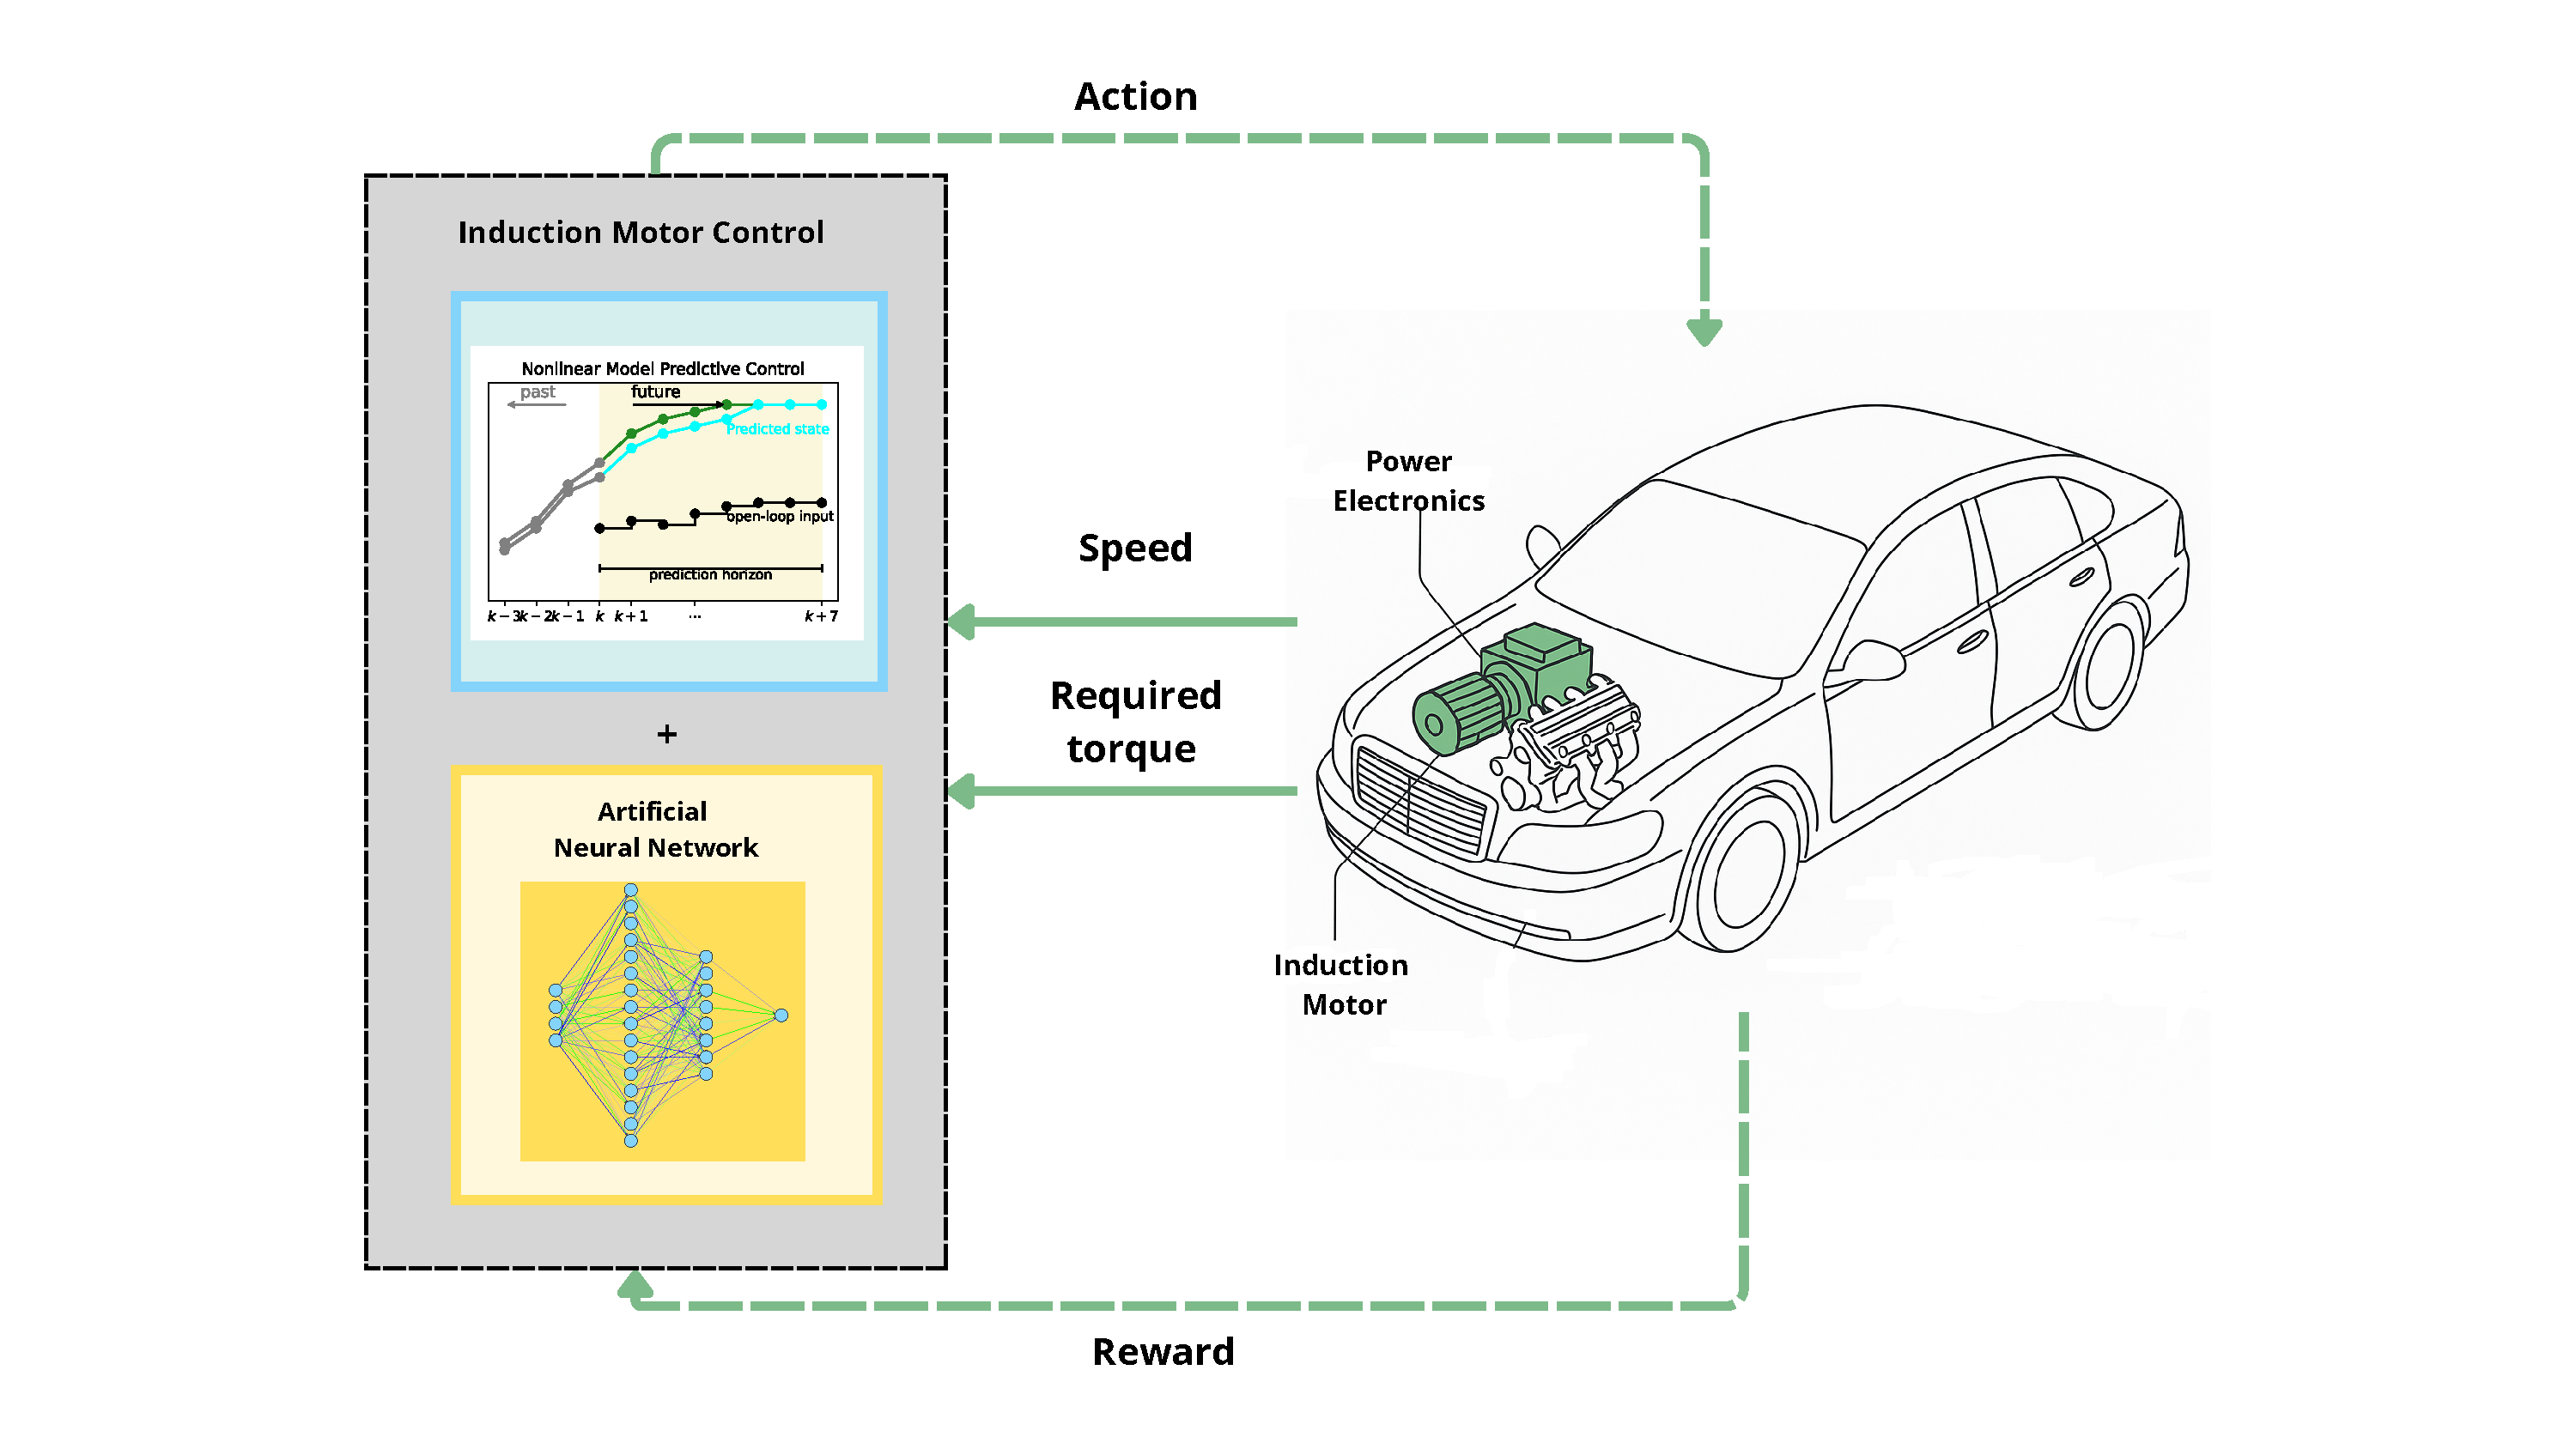
\includegraphics[angle=0, scale=0.45]{Graphical.pdf}
\vspace{8cm}
\end{graphicalabstract}

\begin{highlights}

\item{85 caracteres com espaços}

\item{85 caracteres com espaços}

\item{85 caracteres com espaços}

\item{85 caracteres com espaços}

\item{85 caracteres com espaços}

\end{highlights}

\begin{keyword}
Hierarchical reinforcement learning \sep braking and throttle control \sep nonlinear control \sep hybrid SAC \sep train control optimization
\end{keyword}

\end{frontmatter}

%% \linenumbers
%% main text
\section{Introduction}
\label{sec1}

Heavy haul railways play an important role in economic development by providing an efficient and reliable means of transporting large volumes of heavy and bulk commodities. They are essential for moving minerals, metals, and other raw materials, particularly in resource-rich countries, connecting these products to global markets. By carrying goods in large quantities, heavy haul trains reduce the transportation cost per ton and improve industrial competitiveness.

In addition, this transport mode reduces the burden on road infrastructure, helping to decrease congestion and infrastructure wear. Investments in heavy haul railway systems also create jobs, support the development of remote regions, and encourage technological progress in related areas. As a more sustainable alternative to road transport, heavy haul railways contribute to lower emissions and energy consumption, linking economic growth with environmental responsibility.

Proper braking operation is essential for the safety and efficiency of heavy haul trains. Since these trains transport very large loads over long distances, an adequate braking strategy is required to maintain operational control, especially along track sections with different gradients and terrain conditions. Correct brake application provides more stable deceleration and stopping, reducing the risk of derailment and helping to limit wear on railway infrastructure. Smooth braking can also improve energy use and extend the service life of braking components. In heavy haul operations, where the transported cargo may include hazardous materials, braking reliability is particularly important because it helps protect people, equipment, and the environment. Therefore, the proper use of braking systems is a key aspect of the operational integrity of heavy haul railways.

Pneumatically controlled brake systems remain widely used in heavy haul railway operations in several countries \citep{wei2017air,eckert2023fast}. However, one of the main limitations of this type of system is the delay in brake command propagation along long train composition, since the application signal may take several seconds to reach the rear wagons. This delay can intensify longitudinal impacts at the couplers, as rear freight cars may continue pushing the vehicles ahead before the braking effort is fully developed throughout the train \citep{oprea2013alternative}. A possible alternative to mitigate this limitation is the use of electro-pneumatic valves, which are electronically actuated and allow brake commands to be applied almost simultaneously along the entire consist. In addition, electro-pneumatic systems enable more flexible brake cylinder pressure modulation, including more frequent pressure increases and partial releases, since the brake pipe is no longer used as the direct control medium and can continuously supply air to the freight car reservoirs. Therefore, beyond reducing the delay associated with conventional pneumatic actuation, electro-pneumatic braking creates opportunities for more advanced control strategies. This is particularly relevant for heavy haul train operation, where braking decisions are strongly coupled with traction and dynamic braking actions, and where inappropriate transitions between these modes may affect the longitudinal dynamic response of the train.

\textcolor{Magenta}{This work aims to develop an integrated driving control strategy for heavy freight trains, considering acceleration and braking processes together. The optimal operation of this type of train has been extensively investigated in the literature, especially in relation to energy efficiency, trajectory optimization, smooth driving, operation on downhill sections, and reduction of longitudinal forces between vehicles \citep{lin2017energy,howlett2016new,bai2020multi,wang2019intelligent,zhang2013optimal,yi2022research}. In this context, \cite{eckert2025multi} specifically advanced the optimization of the electro-pneumatic braking process in heavy freight trains, using multi-objective fuzzy control to reduce the energy dissipated during braking and the force peaks in the shock and traction devices. The results obtained by these authors highlighted the potential of optimized control strategies to improve the dynamic performance of the train. However, the approach remained restricted to the braking subsystem. Thus, this work starts from this basis and expands the control problem by including, in the same decision structure, the coordination between traction, dynamic braking, and pneumatic braking. To this end, an approach based on the Hybrid Soft Actor-Critic (SAC) model is adopted, as described by \cite{delalleau2019discretecontinuousactionrepresentation}, allowing the representation of hybrid decisions in which the choice of actuation mode and the intensity of the applied command are treated jointly.}

\textcolor{Magenta}{The integrated formulation of railway operation is directly related to recent advances in automatic train operation systems, known as Automatic Train Operation (ATO). In these systems, traction and braking controls are typically adjusted in a coordinated manner to meet different operational objectives, such as energy efficiency, timetable adherence, comfort, safety, and stopping precision \citep{zhou2020smart,chen2023research,huang2025enhanced}}.

\textcolor{Magenta}{In recent years, machine learning-based methods have been frequently explored in automated train operation systems, as they allow for adjusting traction and braking commands based on interaction with the simulation environment, reducing dependence on predefined speed profiles. \cite{zhou2020smart} proposed intelligent railway operation algorithms based on expert knowledge and reinforcement learning, using Deep Deterministic Policy Gradient (DDPG) and Normalized Advantage Function (NAF), two approaches suitable for continuous control problems, to adjust traction and braking commands in metro systems. Similarly, \cite{huang2025enhanced} combined an expert system and deep learning through reinforcement for the continuous control of traction and braking forces, considering criteria such as safety, comfort, punctuality, stopping precision, and energy efficiency.}

\textcolor{Magenta}{Other recent formulations have also explored different ways of representing the railway control problem. Some studies use Deep Q-Network (DQN), a value-based learning method, to select discrete driving actions, while others employ Proximal Policy Optimization (PPO), a deep reinforcement learning algorithm used in control problems with safety constraints \citep{chen2023research,cheng2024train}. There are also approaches that incorporate reference systems, in which the controller learns to follow or correct a desired trajectory, and studies focused on discrete traction and braking controls, closer to the real operating interfaces of certain trains \citep{shang2021deep,wei2022energy}. Despite these advances, most applications are still concentrated in subways, urban railways, and high-speed trains, whose operating conditions are more controlled and whose train compositions are significantly smaller than those seen in heavy freight trains.}

\textcolor{Magenta}{This difference in application is relevant because operating heavy freight trains imposes more severe dynamic constraints. The train's great length, the high mass transported, the delays associated with the pneumatic system, and the occurrence of significant longitudinal forces make the control problem more sensitive to transitions between traction, relief, dynamic braking, and pneumatic braking \citep{eckert2025multi,wu2023freight}. Therefore, strategies developed for urban systems should be carefully evaluated before being applied to heavy-duty train compositions. In this type of operation, a seemingly adequate control system in terms of operational performance can generate undesirable dynamic responses along the train, especially in the shock and traction devices, whose modeling directly influences the estimation of longitudinal forces on the train composition \citep{eckert2025multi,wu2018parallel,wagner2021review,yadav2023influence,wu2014review}.}

\textcolor{Magenta}{Therefore, detailed modeling of the longitudinal dynamics becomes essential to evaluate the performance of the proposed controller. Adequate representation of the shock and tension devices is important because different formulations of this component can significantly alter the estimation of internal forces in the composition \citep{wu2018parallel,wagner2021review,yadav2023influence,wu2014review}. Similarly, modeling the pneumatic brake system is fundamental to capturing the effects of pressure propagation and its influence on the longitudinal response of the train \citep{wu2023freight}.  
\cite{eckert2025multi} showed that simply replacing conventional pneumatic valves with electro-pneumatic valves, without a proper change in the control strategy, does not guarantee significant improvements in the dynamic behavior of the train. This result reinforces the need to develop controllers capable of exploiting the benefits of electro-pneumatic systems in a coordinated manner with the other operating modes of the train.}

\textcolor{Magenta}{Based on the above, this work proposes a hierarchical learning architecture based on SAC agents for the integrated control of heavy freight train operation. Instead of treating acceleration and braking as independent problems, the proposed approach organizes driving decisions into a common control framework. The proposed structure is organized into two levels: a main agent selects the mode of action to be applied, while subordinate agents determine the intensity of the corresponding command. In this way, the different operating modes available in driving, such as traction, dynamic braking, and pneumatic braking, are addressed within the same decision structure. This organization aims to make the control problem more structured, allowing the decision about the operating mode to be separated from the definition of the magnitude of the applied command.}

\textcolor{Magenta}{Within this framework, the proposed strategy connects the choice of driving mode to the continuous definition of the commands applied to the train. The main contribution of this work, therefore, lies in the development of an integrated control strategy for heavy freight trains, combining hierarchical learning based on SAC agents with detailed dynamic models of the train composition. Unlike approaches focused solely on optimizing braking or trajectory \citep{bai2020multi,eckert2025multi}, the proposed controller dynamically adjusts the available operating modes while driving. The proposed approach is evaluated based on the dynamic response of the train composition, simultaneously considering the effects of traction, dynamic braking, and pneumatic braking on longitudinal forces along the train. This evaluation depends on the adequate representation of longitudinal dynamics and the shock and traction devices. Thus, this work advances beyond approaches focused solely on trajectory or braking optimization, treating train operation as an integrated decision and control problem.}

\textcolor{Magenta}{The rest of this work is divided as follows: Section \ref{Section-Dynamic} presents the train longitudinal dynamics modeling approach, including the detailed model of the pneumatic braking system and the friction-based draft gear model. Section 3 describes the control problem formulation and the proposed hierarchical architecture based on Soft Actor-Critic agents. Section 4 presents the training, validation, and comparison results of the controller under different operational scenarios. Finally, Section 5 summarizes the main conclusions of the work and discusses possible directions for future research.}

\begin{comment}    
\textcolor{red}{PARTE ANTIGA}

\textcolor{red}{Heavy haul railways play a crucial role in developing the economy by offering a reliable and efficient mode of transporting large quantities of heavy and bulk commodities. These railways are the arteries of trade, especially for resource-rich countries, enabling the export of minerals, metals, and other raw materials to global markets. By moving goods in large volumes, heavy haul trains reduce the cost per ton, providing a competitive edge to industries and fostering economic growth. Furthermore, they alleviate pressure on road networks, reducing congestion and wear-and-tear. The infrastructural investment in heavy haul rail networks also generates employment, stimulates development in remote areas, and promotes the advancement of related technologies, which in turn catalyzes industrial innovation and productivity. As a sustainable alternative to road transport, heavy haul railways also contribute to environmental conservation by lowering emissions and energy consumption, aligning economic progress with ecological responsibility.}

\textcolor{red}{Proper train braking operations are vital for the safety and efficiency of heavy haul train operations. Heavy haul trains, which carry massive loads over long distances, rely on scientific braking to maintain control, particularly when navigating varying terrains and gradients. Correct braking ensures steady deceleration and stopping, preventing derailments, and can also contribute to minimizing wear on the rail infrastructure. It also conserves energy, as smooth braking leads to more efficient fuel use and extends the life of braking systems. In the realm of heavy haulage, where cargo often includes hazardous materials, the importance of reliable braking cannot be overstated, as it safeguards both human life and the environment from potential accidents. Therefore, the correct application of braking systems is a critical component in the operational integrity of heavy haul railways.}

\textcolor{red}{The pneumatic-controlled braking system continues to be widely utilized in heavy haul rail transportation across various countries \cite{wei2017air,eckert2023fast}. However, a notable challenge associated with pneumatic control is the delay of several seconds in activating brakes for the rear wagons of lengthy rolling-stocks. This delay results in longitudinal impacts at the couplers, where rear freight cars exert force on the frontal ones \cite{oprea2013alternative}. An effective alternative to address this braking delay involves replacing pneumatic-controlled valves with electro-pneumatic valves. Unlike their pneumatic counterparts, electro-pneumatic valves are electronically controlled, enabling simultaneous activation throughout the entire consist. Furthermore, these valves permit more frequent releases or increases in brake cylinder pressure, as they are not reliant on the brake pipe for control and, therefore, the brake pipe can continuously supply air pressure to the freight cars' reservoirs. The adoption of electro-pneumatic systems also facilitates the implementation of more sophisticated control strategies, enhancing the overall braking process. This can result in minimized dissipated energy and improved safety for the consist, particularly during downhill sections of the railroad.}

\textcolor{red}{This paper focuses on the optimization of the train braking process in the context of heavy haul train driving control. There are still a range of research gaps in this research topic, as reviewed by Lin et al. \cite{lin2017energy}. Both Lin et al. \cite{lin2017energy} and Howlett \cite{howlett2016new} studied the energy issue for freight trains at downhill sections. Bai et al. \cite{bai2020multi} used the Quadratic Programming method to optimize train trajectory for energy efficiency and driving smoothness. Wang et al. \cite{wang2019intelligent} used the machine learning method to reduce in-train forces of heavy haul trains in downhill sections. Zhang et al. \cite{zhang2013optimal} used Model Predictive Control to achieve optimal heavy haul train operation in terms of both in-train forces and energy efficiency. Yi et al. \cite{yi2022research} used a Bald Eagle search algorithm to optimize the freight train operation process.}


\textcolor{red}{It is noted that none of the published studies have included detailed fluid dynamic air brake models in the train braking related optimization process. As reviewed by Wu et al. \cite{wu2023freight}, train air brake models can be classified into three categories: empirical \cite{bosso2023numerical,pfaff2023braking,oprea2013alternative} fluid dynamics \cite{ge2023approach,wei2023influence,wu2017railway,pugi2011preliminary} and fluid-empirical dynamics models \cite{belforte2008numerical,cantone2011traindy,cantone2023simplified,di2017effect}. Fluid dynamics and fluid-empirical dynamics models have the advantages of being high fidelity and adaptive to simulation scenarios. These advantages of greater values for brake related studies as this paper. This paper uses a detailed fluid dynamic air brake model \cite{teodoro2020parallel} and a frictional draft gear model \cite{wu2018parallel}. Different types of draft gear models \cite{wagner2021review,yadav2023influence,wu2014review} have significant influences on in-train force simulations. The detailed frictional draft gear model is then an important element for optimizations that aim to reduce in-train forces. This also represents another innovation of this paper.} 

\textcolor{red}{As previously mentioned, electro-pneumatics enable the implementation of sophisticated control strategies that can be optimized. Among the existing optimizable control strategies, fuzzy logic stands out as a viable solution, demonstrating significant improvements after optimization \cite{da2023aging,da2022dual}. Additionally, it proves to be robust when subjected to conditions different from those in which the controller was initially optimized \cite{silva2022robust}. Consequently, this paper employs a Genetic Algorithm to optimize a fuzzy-based train driving controller. Multiple objectives are considered to reduce in-train forces and energy consumption, thereby enhancing overall train efficiency.}

\textcolor{red}{Following the comprehensive literature review, it is evident that no analogous studies have employed optimization procedures in the context of fuzzy logic control for the electro-pneumatic-based braking process for heavy haul trains, particularly when considering detailed fluid dynamic air brake models in conjunction with the frictional draft gear model for the assessment of in-train forces. As a result of this identified research gap, the primary objective of this paper is to address and bridge this gap in the existing literature.}

\textcolor{red}{Section \ref{Section-Dynamic} will introduce the modelling method for train longitudinal dynamics. This includes the detailed fluid dynamic air brake model and frictional draft gear model. Section 3 presented the method of the brake process optimization. Section 4 presents the optimization results and discussions. Section 5 concludes this paper. }
\end{comment}

\newpage

\section{Train Longitudinal Dynamics} \label{Section-Dynamic}

%\textcolor{red}{REESCREVER A ATUALIZAR AS IMAGENS. TALVEZ RESUMIR E COLOCAR COMO REFERENCIA DE TRAB ANTERIOR}

The simulation framework adopted in this study follows the train longitudinal dynamics formulation described by \cite{cole2006longitudinal}. In this approach, the motion of each vehicle is obtained from the longitudinal force balance, allowing the instantaneous acceleration \(\ddot{x}_n\) [m/s\(^2\)] to be evaluated as a function of the corresponding vehicle mass \(m_n\) [kg]. The train consist analyzed here comprises two Dash9 locomotives placed at the head end, followed by 168 ore freight cars, as illustrated in Fig. \ref{fig:Kinetic}.

\begin{figure}[!h]
  \centering
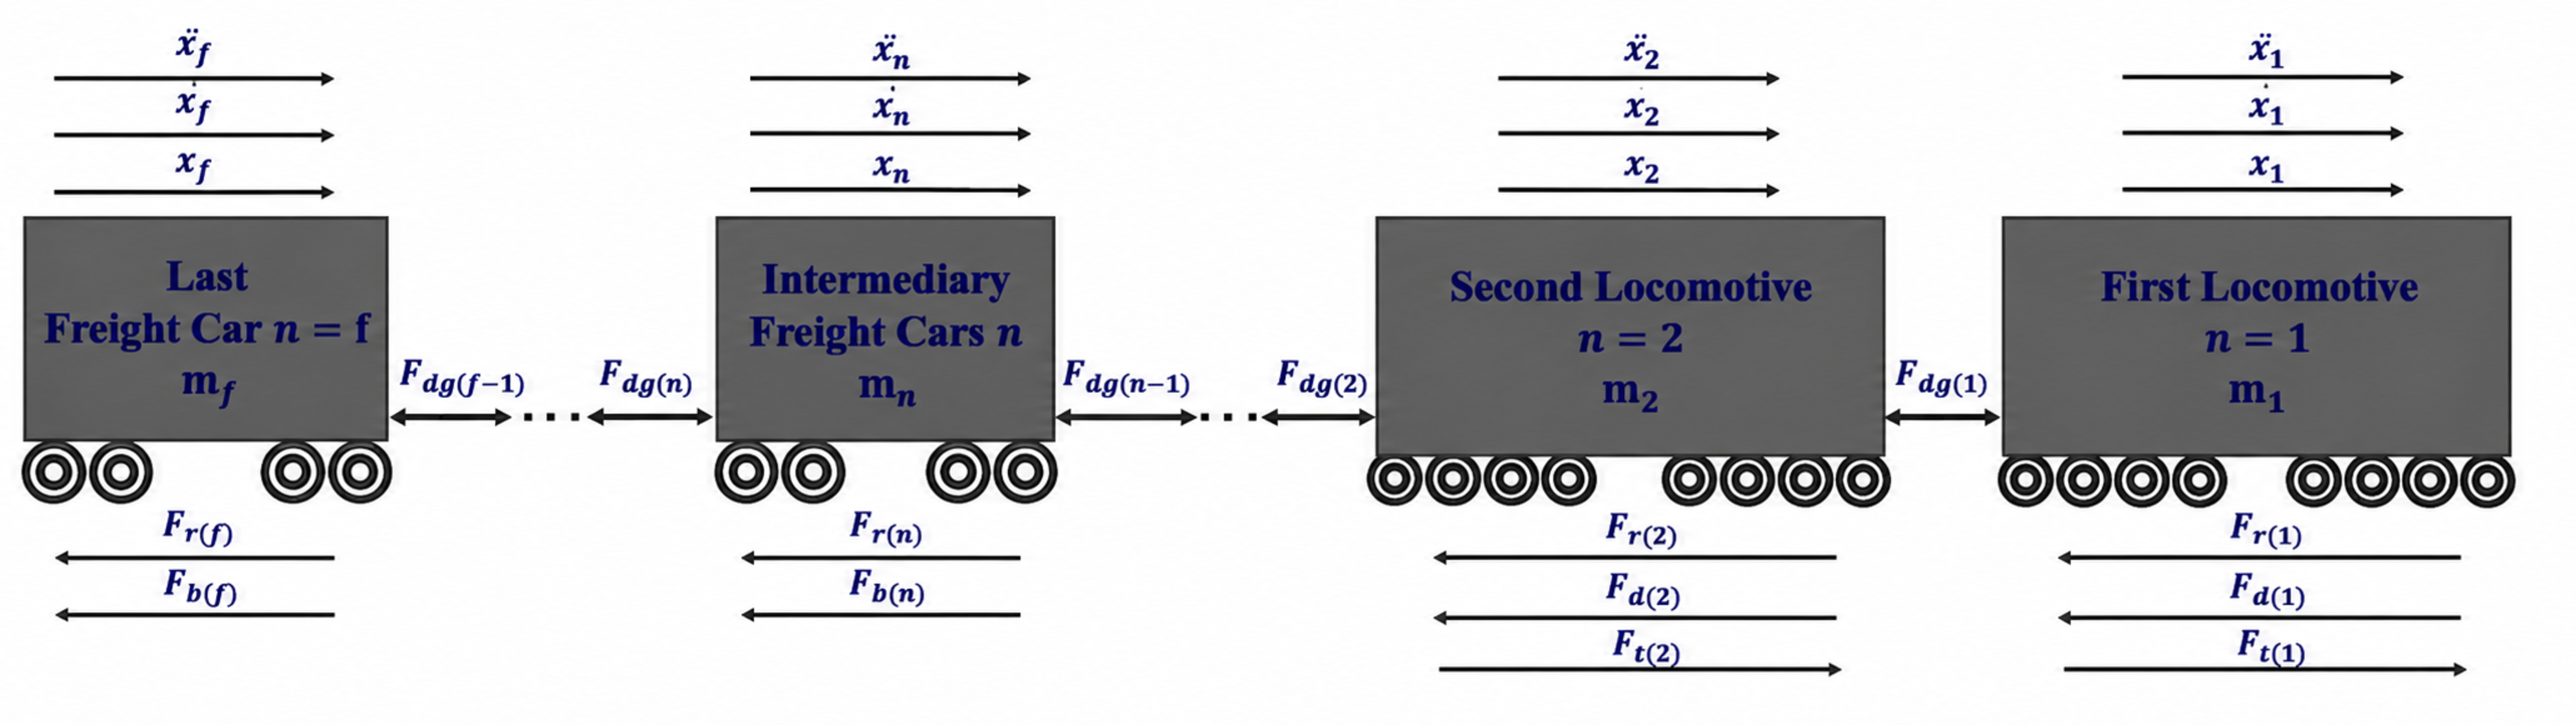
\includegraphics[angle=0, scale=0.250]{DCL_2.pdf}
   \caption{Kinematic representation of the longitudinal train model}
   \label{fig:Kinetic}
 \end{figure}

 \begin{table}[!b]
  \centering
   \caption{Locomotives and freight cars parameter }
       \scalebox{0.9}{
\begin{tabular}{ccccc}
\toprule
\multicolumn{5}{c}{\textbf{Longitudinal train dynamics parameter}s}\tabularnewline
\midrule
\multirow{2}{*}{\textbf{Parameters}} & \multicolumn{2}{c}{\textbf{Locomotives}} & \multicolumn{2}{c}{\textbf{Freight cars}}\tabularnewline
 & $\dot{x_n} \leq 0.1$ & $\dot{x_n} > 0.1$ & $\dot{x_n} \leq 0.1$ & $\dot{x_n} > 0.1$\tabularnewline
 \cmidrule{1-5} 
$A_1$ & 5 & 0.1 & 15 & 0.15\tabularnewline
$A_2$ & 425 & 8.5 & 425 & 4.25\tabularnewline
$B$ & 0 & 0.00938 & 0 & 0.007\tabularnewline
$C$ & 0 & 0.0046 & 0 & 0.000325\tabularnewline
Mass $m_n$ & \multicolumn{2}{c}{$162 \times 10^3$ kg } & \multicolumn{2}{c}{$106.5 \times 10^3$ kg}\tabularnewline
Number of axis $N_a$ & \multicolumn{2}{c}{5} & \multicolumn{2}{c}{4}\tabularnewline
\bottomrule
\end{tabular}  }
  \label{tab:parameters}  
\end{table}



Each vehicle of the train is subjected to a motion resistance force, as defined in Eq. \ref{eq:Frn}. This force accounts for the combined effects of wheel-rail rolling resistance and aerodynamic drag, which are evaluated using the empirical coefficients listed in Table \ref{tab:parameters}. The influence of track geometry is also included in the model by considering the local track gradient, represented by \(\alpha_n\) [rad], and the curve radius \(R_n\) [m].


\begin{equation}\label{eq:Frn}
F_{r\left(n\right)}=m_ng\left(A_{1(n)}+\frac{A_{2(n)}N_{a(n)}}{m_n}+B_n\dot{x}_n+C_n\dot{x}_n^2+sin\alpha_n+ \frac{6.116}{g R_n}\right).
\end{equation}

The longitudinal accelerations of the two head-end locomotives are obtained from the dynamic equilibrium of each vehicle in the longitudinal direction, as expressed by Eqs. \ref{eq:x1} and \ref{eq:x2}.

\begin{equation}\label{eq:x1}
\ddot{x}_1=\frac{F_{t1}-F_{d1}-F_{r1}-F_{dg1}}{m_1},
\end{equation}

\begin{equation}\label{eq:x2}
\ddot{x}_2=\frac{F_{t2}-F_{d2}-F_{r2}+F_{dg1}-F_{dg2}}{m_2},
\end{equation}

\noindent where \(m_1\) and \(m_2\) are the masses of the first and second locomotives, respectively, and \(\ddot{x}_1\) and \(\ddot{x}_2\) are their corresponding longitudinal accelerations. The terms \(F_{t1}\) and \(F_{t2}\) denote the traction forces applied to the locomotives, while \(F_{d1}\) and \(F_{d2}\) represent the dynamic braking forces. The terms \(F_{r1}\) and \(F_{r2}\) are the motion resistance forces defined by Eq. \ref{eq:Frn}. The quantities \(F_{dg1}\) and \(F_{dg2}\) denote the draft-gear forces transmitted through the coupler connections between adjacent vehicles.

The traction and dynamic braking forces are defined according to the train control schedule, which specifies the operating condition of each Dash9 locomotive. In traction mode, the force \(F_{t(n)}\)~[N] is obtained from the tractive-effort curves associated with the eight power notches, from \(P_1\) to \(P_8\), as shown in Fig. \ref{fig:LOCO}a. In dynamic braking mode, the force \(F_{d(n)}\)~[N] follows the four braking stages, from \(D_1\) to \(D_4\), as illustrated in Fig. \ref{fig:LOCO}b. After these locomotive forces are defined, the resulting acceleration also depends on the draft gear forces \(F_{dg(n)}\)~[N], which represent the interaction between adjacent vehicles and are discussed in Section \ref{Draft}.


\begin{figure}[!h]
  \centering
   \subfigure[Traction]{{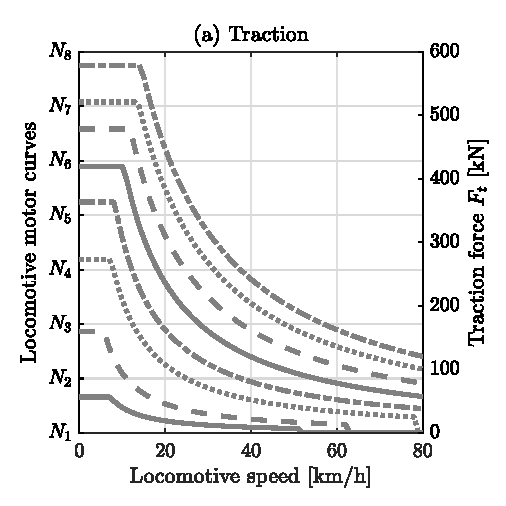
\includegraphics[angle=0, scale=0.89]{TRACTION_FORCE.eps}}}
   \subfigure[Dynamics braking]{{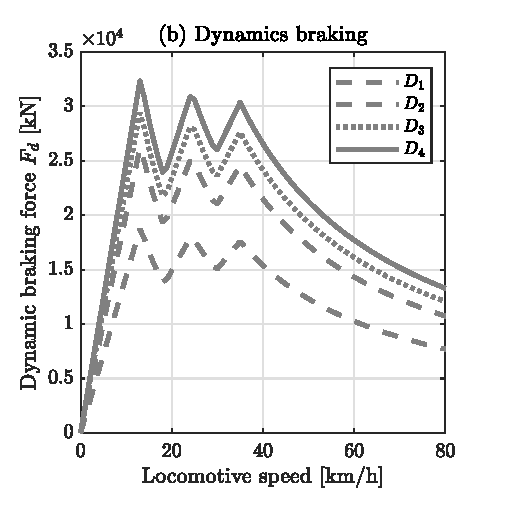
\includegraphics[angle=0, scale=0.89]{DYNAMIC_BREAK_FORCE.eps}}}
   \caption{Locomotive traction and dynamic brake curves \textcolor{red}{refiz a figura numa escala de cinza}}
   \label{fig:LOCO}
 \end{figure}

The acceleration of the intermediate freight cars, \(\ddot{x}_n\), is obtained from Eq.~\ref{eq:xn}. This equation accounts for the longitudinal forces acting on the \(n\)-th car, namely the draft-gear forces at the front and rear ends, \(F_{dg(n-1)}\) and \(F_{dg(n)}\), the motion resistance force, \(F_{r(n)}\), and the pneumatic braking force, \(F_{b(n)}\). The pneumatic braking model adopted in this study is described in Section~\ref{Brake}. Similarly, the acceleration of the last freight car, \(\ddot{x}_f\), is calculated using Eq.~\ref{eq:xf}.

\begin{equation}\label{eq:xn}
\ddot{x}_n=\frac{-F_{r(n)}-F_{bn}+F_{dg(n-1)}-F_{dg(n)}}{m_n},
\end{equation}

\begin{equation}\label{eq:xf}
\ddot{x}_f=\frac{{-F}_{r(f)}-F_{b\left(f\right)}+F_{dg(f-1)}}{m_f}.
\end{equation}


Once the instantaneous accelerations, \(\ddot{x}_n\)~[m/s\(^2\)], are computed, they are numerically integrated using the Matlab/Simulink\texttrademark\ ODE1 solver to obtain the velocity, \(\dot{x}_n\)~[m/s], and displacement, \(x_n\)~[m], of each car. The use of ODE1 is justified by the small time step, \(\Delta t \leq 0.0005\)~s, required by the brake pipe airflow simulation, and its accuracy has been shown to be comparable to higher-order solvers, such as ODE4 and ODE8 \citep{eckert2019dissipated}.

\subsection{Draft gear model}\label{Draft}

The draft gear forces, denoted by $F_{dg(n)}$, are determined using the model proposed by \cite{wu2017comparisons}. This model is coupled with the dissipated-energy approximation method \cite{eckert2019dissipated,eckert2023fast}, which is applied during the transition between the loading and unloading phases to improve the computational efficiency of the simulations. The adopted formulation accounts for the main mechanical components of the draft gear and their corresponding geometrical characteristics, as illustrated in Fig. \ref{fig:Draftgear}. The resulting force--displacement relationships are given by

\begin{figure}[!h]
\centering
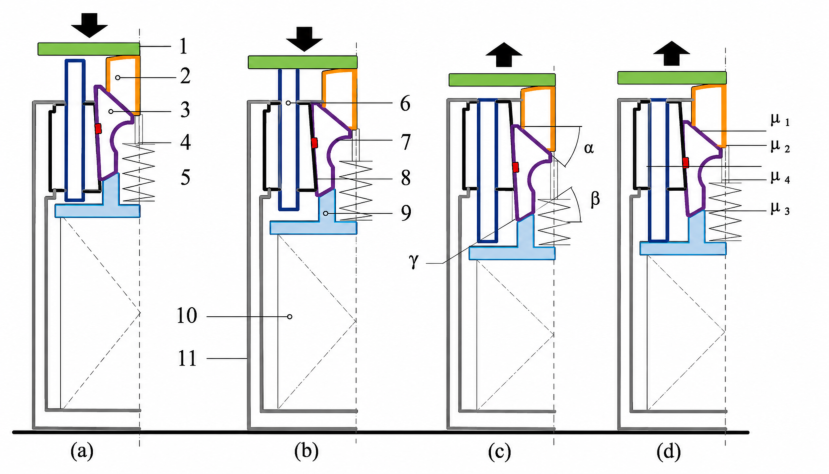
\includegraphics[angle=0, scale=1.2]{draftgear model.pdf}
\caption{Friction draft gear model: (a) loading stage 1, (b) loading stage 2, (c) unloading stage 1, and (d) unloading stage 2; 1 -- follower, 2 -- central wedge, 3 -- wedge shoe, 4 -- release spring, 5 -- outer stationary plate, 6 -- movable plate, 7 -- lubricating metal, 8 -- inner stationary plate, 9 -- spring seat, 10 -- main springs, and 11 -- housing.}
\label{fig:Draftgear}
\end{figure}

\begin{equation}
\label{eq:DRAF1}
F_{j,i}
=
\Psi_i F_{sm}
-
\left(\Psi_i - 1\right)F_{sr},
\qquad i=1,\ldots,4,
\end{equation}

\noindent where, $F_{j,i}$ represents the draft gear force associated with the $i$-th operating stage, where $i=1,\ldots,4$. The terms $F_{sm}$ and $F_{sr}$ denote the main spring force and the release spring force, respectively. The parameter $\Psi_i$ is defined as the force amplification factor, accounting for the effects of wedge geometry and frictional contact within the draft gear mechanism.

Since the mechanical response of the draft gear varies throughout the loading and unloading stages, $\Psi_i$ must be evaluated according to the corresponding operating condition. The force amplification factors $\Psi_i$ are defined as


\begin{equation}
\label{eq:DRAF2}
\Psi_1
=
\frac{
1+
\tan\left(\beta+\arctan\left(\mu_3\right)\right)
\tan\left(\gamma+\arctan\left(\mu_1\right)\right)
}{
1-
\tan\left(\alpha+\arctan\left(\mu_2\right)\right)
\tan\left(\gamma+\arctan\left(\mu_1\right)\right)
},
\end{equation}

\begin{equation}
\label{eq:DRAF3}
\Psi_2
=
\Psi_1
+
\frac{
2\left[1-\mu_1\tan\left(\gamma\right)\right]\mu_4
\left(\Psi_1-1\right)
}{
\mu_1+\tan\left(\gamma\right)
},
\end{equation}

\begin{equation}
\label{eq:DRAF4}
\Psi_3
=
\frac{
1+
\tan\left(\beta-\arctan\left(\mu_3\right)\right)
\tan\left(\gamma-\arctan\left(\mu_1\right)\right)
}{
1-
\tan\left(\alpha-\arctan\left(\mu_2\right)\right)
\tan\left(\gamma-\arctan\left(\mu_1\right)\right)
},
\end{equation}

\noindent and
\begin{equation}
\label{eq:DRAF5}
\Psi_4
=
\frac{
\left[\tan\left(\gamma\right)-\mu_1\right]\Psi_3
}{
\tan\left(\gamma\right)
\left[
1-2\mu_1\mu_4+2\mu_1\mu_4\Psi_3
\right]
+
2\mu_4\Psi_3
-
2\mu_4
-
\mu_1
},
\end{equation}

\noindent where $\alpha$, $\beta$, and $\gamma$ are the wedge angles indicated in Fig. \ref{fig:Draftgear}, while $\mu_1$ to $\mu_4$ are the friction coefficients associated with the corresponding contact interfaces.

\textcolor{Magenta}{The friction coefficients between the components, $\mu_i$, are calculated using the exponential formulation presented by \cite{berger2002friction} and later applied by \cite{wu2014review} to represent the peak force behavior of friction draft gears. In this formulation, $\mu_i$ varies as a function of the relative velocity $v_i$, allowing the friction behavior to transition between static and dynamic conditions. The parameter $\sigma$ defines the sensitivity of this variation with respect to velocity. The friction coefficient is then given by}

\begin{equation}
\label{eq:friction_coefficient}
\mu_i
=
\mu_s
+
\left(\mu_s-\mu_k\right)
\exp\left(-\sigma |v_i|\right),
\end{equation}

\noindent \textcolor{Magenta}{where $\mu_s$ and $\mu_k$ are the static and dynamic friction coefficients, respectively, $v_i$ is the relative velocity at the corresponding contact interface, and $\sigma$ controls how rapidly $\mu_i$ changes with variations in $v_i$.}

\textcolor{Magenta}{After defining the friction coefficients, the relative velocities at the contact interfaces are obtained from the follower velocity of the draft gear. These velocities are required because the friction coefficients $\mu_i$ depend on the relative motion between the contacting components. Based on the geometry of the mechanism, the relative velocities $v_1$, $v_2$, $v_3$, and $v_4$ are expressed as functions of the wedge angles $\alpha$, $\beta$, and $\gamma$, and of the follower velocity $v_f$, as follows:}

\begin{equation}
\label{eq:relvel1}
v_1
=
\frac{\cos(\alpha)}
{\cos(\alpha+\gamma)}
v_f ,
\end{equation}

\begin{equation}
\label{eq:relvel2}
v_2
=
\frac{\sin(\gamma)}
{\cos(\alpha+\gamma)}
v_f ,
\end{equation}

\begin{equation}
\label{eq:relvel3}
v_3
=
\frac{\cos(\alpha)\sin(\gamma)}
{\cos(\alpha+\gamma)\cos(\beta)}
v_f ,
\end{equation}

\begin{equation}
\label{eq:relvel4}
v_4(j)
=
\begin{cases}
\dfrac{\cos(\alpha)\sin(\gamma)}
{\cos(\alpha+\gamma)\cos(\beta)}
v_f, & j=4,\\
v_f, & j=2,\\
0, & j=1 \text{ or } j=3.
\end{cases}
\end{equation}

It is worth noting that the four values of the index $i$ in Eqs. \eqref{eq:DRAF1} and \eqref{eq:friction_coefficient} correspond to the four contact interactions considered in the draft gear working process, as illustrated in Fig. \ref{fig:Draftgear}. The first and second stages are associated with loading, whereas the third and fourth stages describe unloading. Specifically, the first loading stage occurs before the follower comes into contact with the movable plates, while the second loading stage corresponds to the downward motion of these plates. During unloading, the first stage takes place before the spring seat contacts the movable plates, whereas the second unloading stage corresponds to their upward motion. In the present simulations, the model parameters were defined based on the MARK50 draft gear, following the methodology reported in \cite{eckert2023fast}.






The transition between loading and unloading conditions was treated using the dissipated-energy approximation approach reported in \cite{eckert2019dissipated,eckert2023fast}. With this procedure, the coupler force is selected according to the current contact condition and the transition state, as expressed by

\begin{equation}
\label{eq:energy}
F_c
=
\begin{cases}
0, & \text{within couplers slack}, \\[2mm]
\dfrac{F_c(t-dt)+F_j(t)}{2}, & \text{for a loading--unloading transition}, \\[3mm]
F_j(t), & \text{for all other cases}.
\end{cases}
\end{equation}

\noindent where $F_c$ represents the coupler force evaluated at the current time instant. The variable $t$ denotes time, while $dt$ corresponds to the numerical time increment adopted in the simulation. The term $F_j(t)$ is the draft gear force computed from the force--displacement formulation described above. Further information on the draft gear formulation and its implementation is available in \cite{wu2017comparisons} and  \cite{eckert2019dissipated,eckert2023fast}.

\subsection{Pneumatic Brake System}\label{Brake}

The pneumatic brake system is commonly classified into two main configurations: the automatic pneumatic brake system and the electro-pneumatic brake system. In the automatic pneumatic brake system, braking is commanded by pressure variations in the brake pipe, which links the brake components distributed along the train consist. When a pressure reduction occurs in the brake pipe, the control valve, such as the ABDX or DB-60 valves commonly used in railway applications, detects this change and initiates the brake application by connecting the wagon reservoir to the brake cylinders.

Brake release is achieved by increasing the pressure in the brake pipe. This pressure rise changes the operating condition of the control valve, allowing the brake cylinders to exhaust to the atmosphere while the wagon reservoirs are recharged through the brake pipe. One of the main limitations of this system is the delay in brake command transmission, since the application signal depends on the propagation of the pressure reduction along the pipe. In addition, the system is not well suited for repeated sequences of brake application and release, because the reservoirs in each wagon require time to recover their maximum operating pressure. Mathematical models for this type of brake system are presented by \cite{pugi2013design} and  \cite{teodoro2019fast}.

The electro-pneumatic brake system employs electrical commands to control brake application and release along the train consist. In the present study, the system is represented using an EP60 module, which consists of an independent set of electro-pneumatic valves coupled to a conventional pneumatic brake control valve, such as the ABDX or DB-60. This module governs the pneumatic connections involved in the braking process by linking the emergency reservoir to the corresponding brake cylinder during brake application and by connecting the brake cylinder to the atmosphere during brake release. The electro-pneumatic brake model adopted in this work is shown in Fig. \ref{fig:Brake-model} and was implemented based on the brake schematic and formulation proposed by \cite{teodoro2019fast}.

\begin{figure}[!h]
  \centering
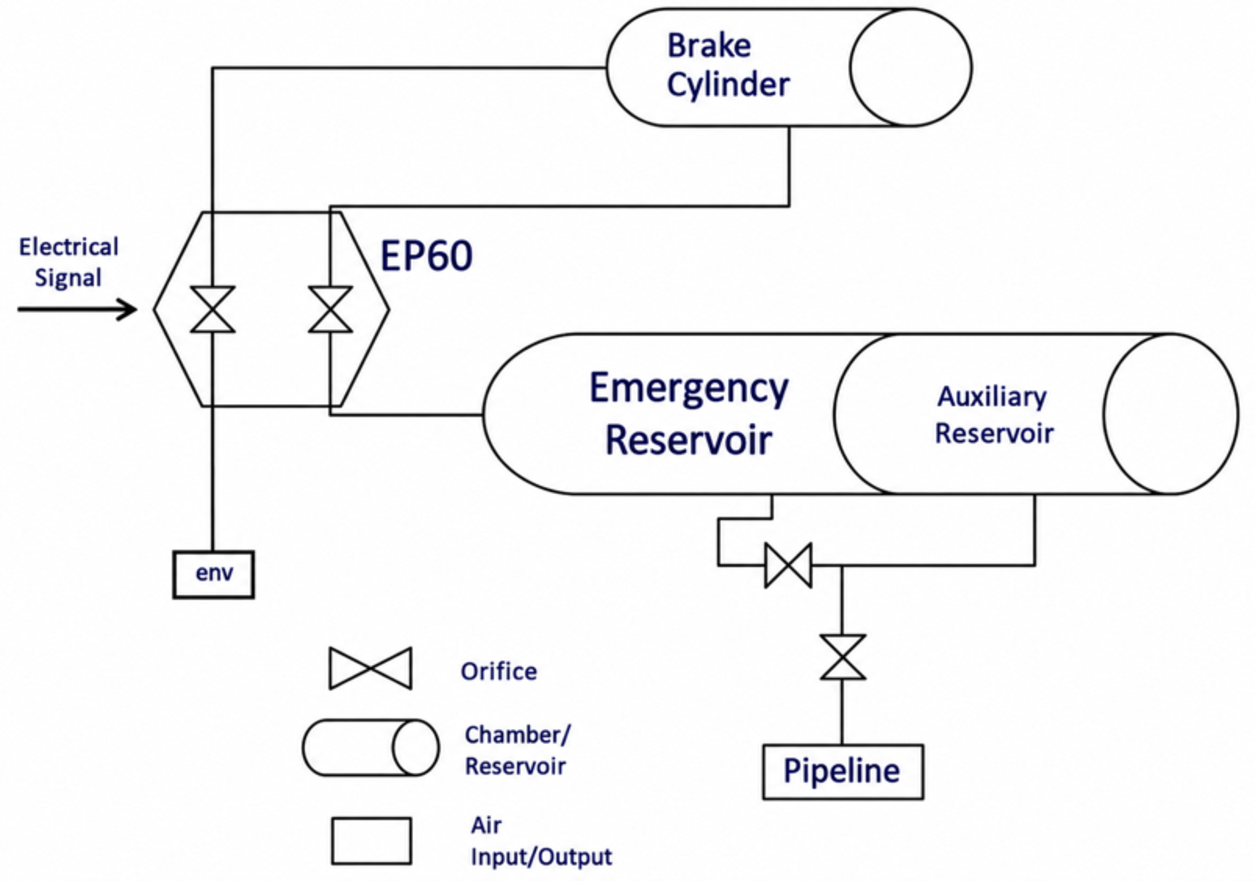
\includegraphics[scale=0.57]{pneumatico.pdf}
   \caption{Brake model schematic}
   \label{fig:Brake-model}
 \end{figure}

The brake system is commanded by the driver, who sets the desired pressure through the locomotive control system. Based on this command, electrical signals are transmitted from the locomotive to all wagons through a wired connection between the electro-pneumatic valves, with negligible transmission delay. These signals are interpreted by the EP60 control module, which changes the pneumatic connections in each wagon to apply or release the braking force.

During brake application, the EP60 module connects the emergency reservoir to the brake cylinder, allowing the cylinder to be pressurized until the commanded pressure level is reached. During brake release, the module connects the brake cylinder to the atmosphere, reducing its pressure until it reaches the value specified by the control signal. At the same time, the brake pipe continuously supplies the auxiliary and emergency reservoirs, keeping their pressures close to the maximum operating level. As a result, partial releases and successive brake application--release sequences can be performed without reducing the braking capability of the system.


The electro-pneumatic brake system is modeled based on the formulation proposed by \cite{pugi2013design}. In this approach, pressure losses between connected pneumatic components are represented by orifices, whereas the compressed-air volumes are modeled as chambers, in which the pressure of each component is evaluated. The brake pipe is also discretized as a series of interconnected chambers and orifices. As discussed by \cite{teodoro2019fast}, this modeling strategy provides satisfactory results while requiring a lower computational cost than more detailed approaches.

\begin{comment}
\textcolor{red}{The simulation model is based on the train longitudinal dynamics present in \cite{cole2006longitudinal}, in which the sum of the forces applied in each freight car is used to define the resulting instantaneous acceleration $\ddot{x_n}$ [m/s$^2$] according to the car mass $m_n$ [kg]. The analysed rolling-stock is composed of two Dash9 locomotives located ahead of 168 ore freight cars as shown the Fig. \ref{fig:Kinetic}.}

\begin{figure}[!h]
  \centering
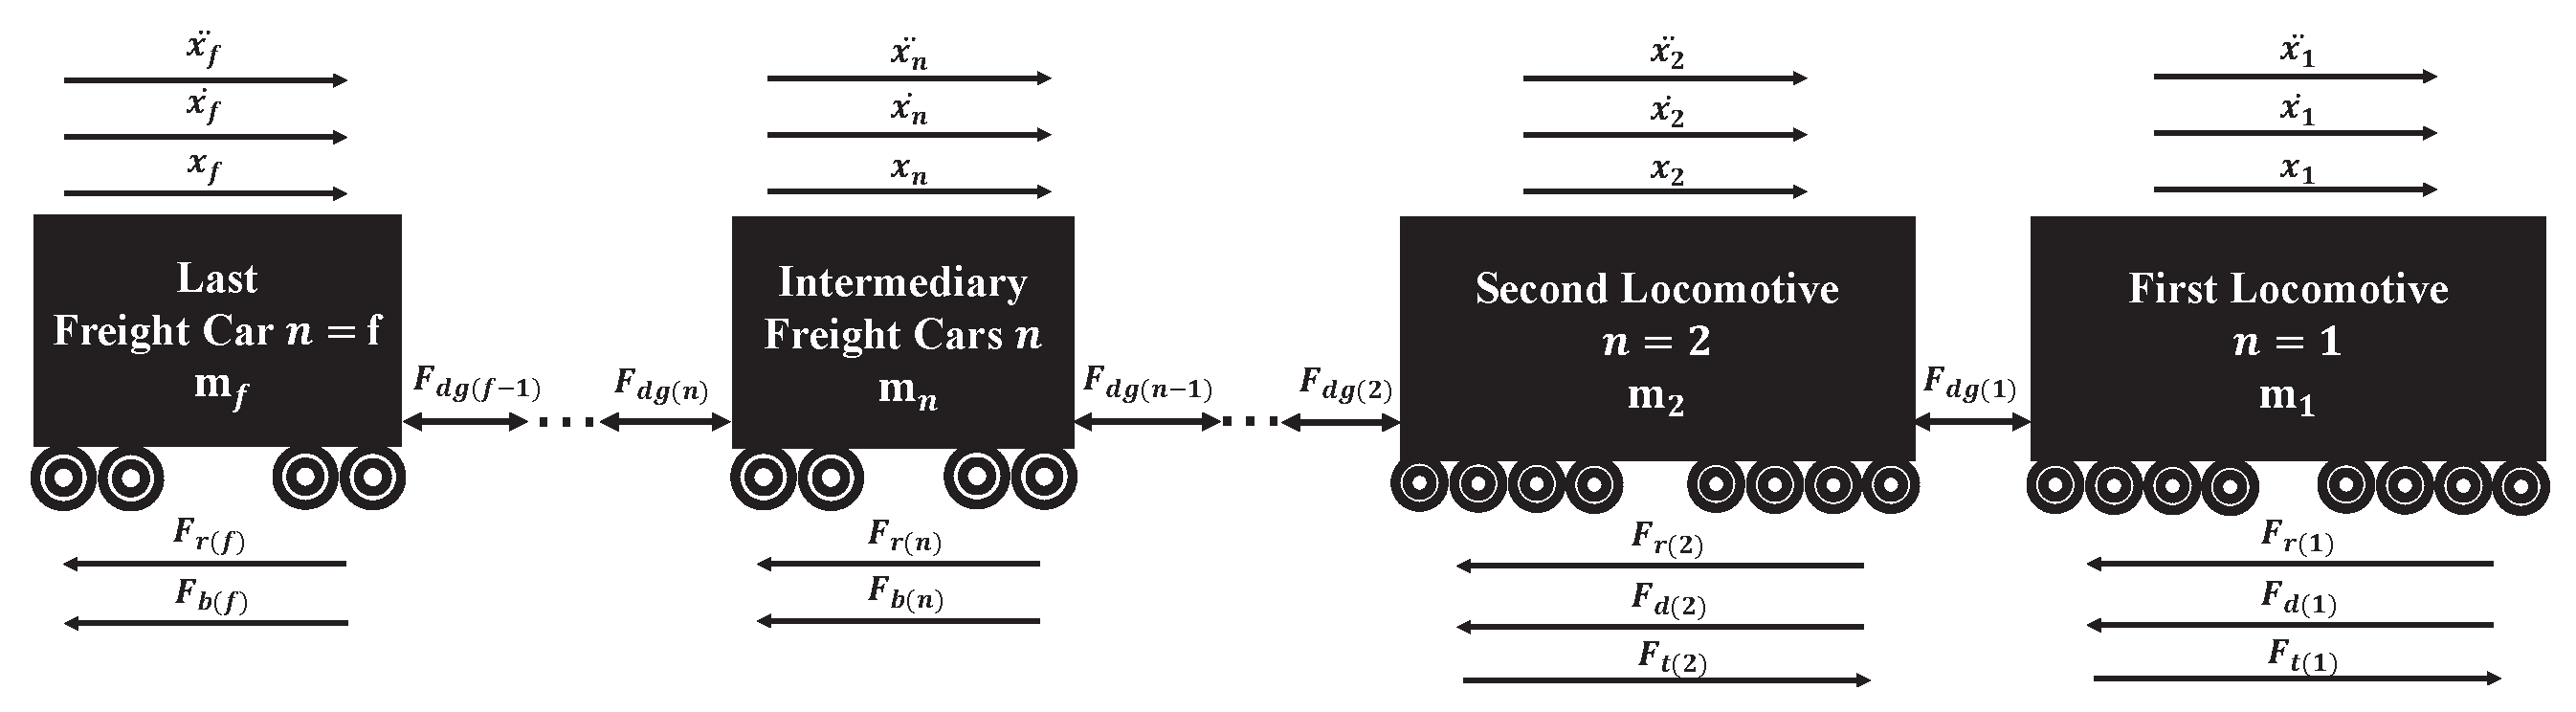
\includegraphics[angle=0, scale=0.31]{DCL.eps}
   \caption{Kinetic diagram}
   \label{fig:Kinetic}
 \end{figure}

 \begin{table}[!b]
  \centering
   \caption{Locomotives and freight cars parameter }
       \scalebox{0.9}{
\begin{tabular}{ccccc}
\toprule
\multicolumn{5}{c}{\textbf{Longitudinal train dynamics parameter}s}\tabularnewline
\midrule
\multirow{2}{*}{\textbf{Parameters}} & \multicolumn{2}{c}{\textbf{Locomotives}} & \multicolumn{2}{c}{\textbf{Freight cars}}\tabularnewline
 & $\dot{x_n} \leq 0.1$ & $\dot{x_n} > 0.1$ & $\dot{x_n} \leq 0.1$ & $\dot{x_n} > 0.1$\tabularnewline
 \cmidrule{1-5} 
$A_1$ & 5 & 0.1 & 15 & 0.15\tabularnewline
$A_2$ & 425 & 8.5 & 425 & 4.25\tabularnewline
$B$ & 0 & 0.00938 & 0 & 0.007\tabularnewline
$C$ & 0 & 0.0046 & 0 & 0.000325\tabularnewline
Mass $m_n$ & \multicolumn{2}{c}{$162 \times 10^3$ kg } & \multicolumn{2}{c}{$106.5 \times 10^3$ kg}\tabularnewline
Number of axis $N_a$ & \multicolumn{2}{c}{5} & \multicolumn{2}{c}{4}\tabularnewline
\bottomrule
\end{tabular}  }
  \label{tab:parameters}  
\end{table}



\textcolor{red}{All rolling-stock cars are submitted to their respective movement resistance force defined in Eq. \ref{eq:Frn}, that englobe the wheel–rail rolling resistance and the aerodynamic drag, defined according to the empirical coefficients presented in the Table \ref{tab:parameters}. Moreover, the railroad geometry influence is also considered according to the railroad slope angle $\alpha_n$ [rad] and the curves' radii $R_n$ [rad].}


\begin{equation}\label{eq:Frn}
F_{r\left(n\right)}=m_ng\left(A_{1(n)}+\frac{A_{2(n)}N_{a(n)}}{m_n}+B_n\dot{x}_n+C_n\dot{x}_n^2+sin\alpha_n+ \frac{6.116}{g R_n}\right)
\end{equation}

\textcolor{red}{The first and second locomotive accelerations are defined by Eqs. \ref{eq:x1} and \ref{eq:x2} respectively, as a function of the train control schedule, that defines the applied traction $F_{t(n)}$~[N] among the 8 available notches ($P_1$ to $P_8$) curves for the Dash9 locomotives according to Fig. \ref{fig:LOCO}a, or dynamic braking $F_{d(n)}$ [N] forces, which convert a portion of the kinetic energy into heat to be dissipated according to the 4 available stages ($D_1$ to $D_4$), as shown in Fig. \ref{fig:LOCO}b.}

\begin{equation}\label{eq:x1}
\ddot{x}_1=\frac{F_{t1}-F_{d1}-F_{r1}-F_{dg1}}{m_1}
\end{equation}

\begin{equation}\label{eq:x2}
\ddot{x}_2=\frac{F_{t2}-F_{d2}-F_{r2}+F_{dg1}-F_{dg2}}{m_2}
\end{equation}

\begin{figure}[!b]
  \centering
   \subfigure[Traction]{{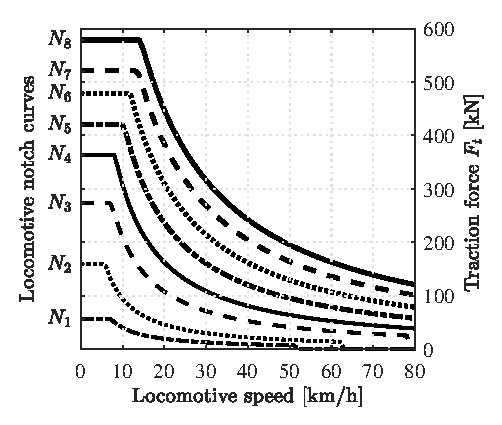
\includegraphics[angle=0, scale=0.89]{LOCO1.eps}}}
   \subfigure[Dynamics braking]{{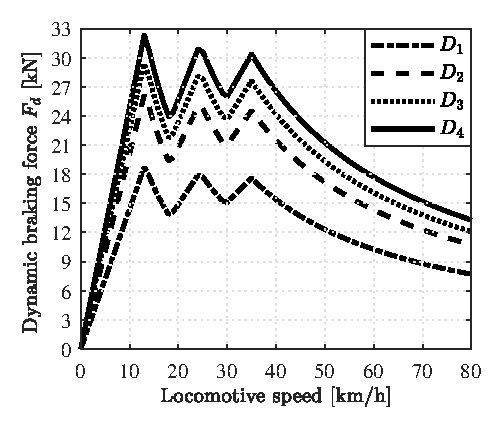
\includegraphics[angle=0, scale=0.89]{LOCO2.eps}}}
   \caption{Locomotive traction and dynamic brake curves}
   \label{fig:LOCO}
 \end{figure}


\textcolor{red}{Once the locomotive traction or dynamic braking forces are defined, the resulting acceleration is defined as a function of its respective draft gear forces $F_{dg(n)}$ [N] that represent the interaction between two connected cars and will be properly discussed in section \ref{Draft}.}

\textcolor{red}{The intermediary freight cars accelerations $\ddot{x}_n$ are defined by the Eq. \ref{eq:xn}, as the sum of the frontal ($F_{dg(n-1)}$) and rear ($F_{dg(n)}$) draft gear forces, the respective rolling resistance ($F_{r(n)}$) and the braking force $F_{b(n)}$ [N] applied by the wagons pneumatic braking system, that will be presented in section \ref{Brake}. Finally, the last freight car acceleration $\ddot{x}_f$ is calculated by Eq. \ref{eq:xf}.}


\begin{equation}\label{eq:xn}
\ddot{x}_n=\frac{-F_{r(n)}-F_{bn}+F_{dg(n-1)}-F_{dg(n)}}{m_n}
\end{equation}

\begin{equation}\label{eq:xf}
\ddot{x}_f=\frac{{-F}_{r(f)}-F_{b\left(f\right)}+F_{dg(f-1)}}{m_f}
\end{equation}


\textcolor{red}{Once all instantaneous accelerations $\ddot{x}_n$ [m/s$^2$] are defined they are numerically integrated by the Matlab/Simulink\texttrademark\ ODE1 (Euler) integrator, to define each car speed $\dot{x}_n$~[m/s] and displacement $x_n$ [m]. The use of ODE1 to solve the train dynamics is allowed due to the small-time steps ($\Delta_t \leq 0.0005$ s) required by the brake pipe airflow simulation. Furthermore, as shown in \cite{eckert2019dissipated}, the ODE1 showed similar results when compared to high order integrators such as ODE4 (Runge–Kutta) and ODE8 (Dormand–Prince).}

\subsection{Draft gear model}\label{Draft}



\textcolor{red}{The draft gear forces $F_{dg(n)}$ are defined by the model presented by Wu et al.  \cite{wu2017comparisons}, combined with the dissipated energy approximation method \cite{eckert2019dissipated,eckert2023fast} applied in the transition between the loading and unloading stages, to enhance the computational efficiency. The draft gear model has considered all key components and their geometries (Fig. \ref{fig:Draftgear}). The force-displacement characteristics are expressed as:}

\begin{equation}\label{eq:DRAF1}
F_{j,i}=\mathrm{\Psi}_iF_{sm}-\left(\mathrm{\Psi}_i-1\right)F_{sr},\ \ \left(i=1,\ 4\right)
\end{equation}

\begin{equation}\label{eq:DRAF2}
\mathrm{\Psi}_1=\frac{1+tan\left(\beta+arctan\left(\mu_3\right)\right)tan\left(\gamma+arctan\left(\mu_1\right)\right)}{1-tan\left(\alpha+arctan\left(\mu_2\right)\right)tan\left(\gamma+arctan\left(\mu_1\right)\right)}
\end{equation}

\begin{equation}\label{eq:DRAF3}
\mathrm{\Psi}_2=\mathrm{\Psi}_1+\frac{2\left(1-\mu_1tan\left(\gamma\right)\right)\mu_4\left(\mathrm{\Psi}_1-1\right)}{\mu_1+tan(\gamma)}
\end{equation}

\begin{equation}\label{eq:DRAF4}
\mathrm{\Psi}_3=\frac{1+tan\left(\beta-arctan\left(\mu_3\right)\right)tan\left(\gamma-arctan\left(\mu_1\right)\right)}{1-tan\left(\alpha-arctan\left(\mu_2\right)\right)tan\left(\gamma-arctan\left(\mu_1\right)\right)}
\end{equation}

\begin{equation}\label{eq:DRAF5}
\mathrm{\Psi}_4= \frac{\left(tan (\gamma)-\mu_1\right) \mathrm{\Psi}_3}{tan (\gamma) \left(1-2\mu_1\mu_4+2\mu_1\mu_4 \mathrm{\Psi}_3\right)+2\mu_4\mathrm{\Psi}_3-2\mu_4-\mu_1}
\end{equation}
\textcolor{red}{where $F_{j,i}$ is the draft gear force; $i\ \left(i=1,\ 4\right)$ indicates different stage of the draft gear working process; $\mathrm{\Psi}_i$ is the force amplifying factor; $F_{sm}$ is the main spring force; $F_{sr}$ is the release spring force; $\alpha$, $\beta$, and $\gamma$ are wedge angles as shown in Fig. \ref{fig:Draftgear}; and $\mu_1- \mu_4$ are coefficients of friction that are also shown in Fig. \ref{fig:Draftgear}. It can be seen that the model considered four stages of the working process: two loading stages and two unloading stages. The first loading stage describes the period before the follower touches the movable plates. The second loading stage describes the period corresponding to the downward movements of the movable plates. The first unloading stage represents the period before the spring seat touches the movable plates. The second unloading stage represents the period when movable plates are moving upwards. The simulation utilized coefficients derived from the MARK50 draft gear, following the methodology outlined in a prior study \cite{eckert2023fast}.}







\textcolor{red}{To handle the transitions between any loading and unloading stage, a Dissipated Energy Model \cite{eckert2019dissipated,eckert2023fast} was used: }

\begin{equation}\label{eq:energy}
F_c=\left\{\begin{matrix}0 & \text{within coupler slack}\\\dfrac{F_c\left(t-dt\right)+F_j(t)}{2}& \text{transition}\\F_j& \text{otherwise}\\\end{matrix}\right.
\end{equation}
\textcolor{red}{where $F_c$ is the current step of coupler force; $t$ is time; $dt$ is the simulation time step-size; and $F_j$ is the previously calculated draft gear force. More details about the draft gear model can be found in Wu et al. \cite{wu2017comparisons} and Eckert et al. \cite{eckert2019dissipated,eckert2023fast}. }


\subsection{Pneumatic Brake System}\label{Brake}

\textcolor{red}{The pneumatic brake system can be separated into two categories, automatic pneumatic brake system and electro-pneumatic brake systems. The automatic pneumatic brake system is activated by the pressure variation in the brake pipeline, which connects all brake components through the composition. Whenever the pressure drops, a control valve (ABDX or DB-60, names of the commonly used control valves) identifies this pressure change and applies brake force, connecting a reservoir located in the wagon to its brake cylinders. To release the brake force, an increase in the pipeline pressure activates the control valve, and it connects the brake cylinder to the environment to completely depressurize it and connects the pipeline to the wagon reservoirs to pressurize them. This type of brake has a delay in the application signal due to the pressure drop propagation speed through the pipeline, and it does not support several sequences of brake applications and release, since it needs time to pressurize the reservoirs in each wagon to the maximum work pressure. Models to represent this type of brake system are presented by Pugi et al. \cite{pugi2013design} and \mbox{Teodoro et al. \cite{teodoro2019fast}.}}

\textcolor{red}{The electro-pneumatic brake system uses electrical signals to apply or release brakes in railway composition. The system evaluated in this work uses an EP60, which is composed of a segregated module of electro-pneumatic valves connected to a commonly used pneumatic brake control valve, such as ABDX or DB-60. This module is responsible for connecting the emergency reservoir to its responsible brake cylinder and the brake cylinder to the environment. Figure \ref{fig:Brake-model} presents the electro-pneumatic brake model implemented based on Teodoro et al. \cite{teodoro2019fast} brake schematic and model.}

\begin{figure}[!h]
  \centering
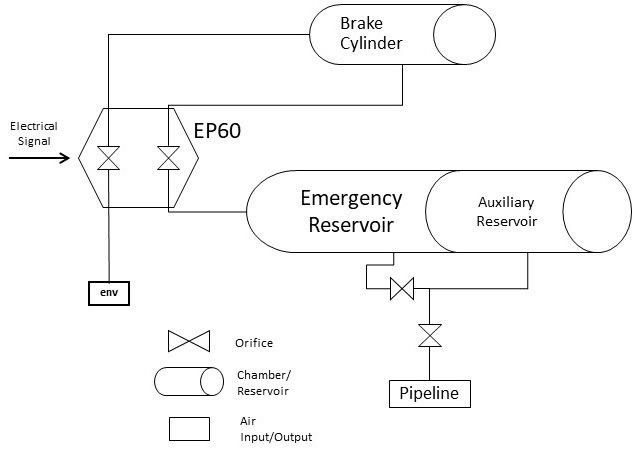
\includegraphics[scale=0.57]{brake-model.jpg}
   \caption{Brake model schematic}
   \label{fig:Brake-model}
 \end{figure}

\textcolor{red}{The driver controls the brake system, setting up the desirable pressure in the locomotive control. This procedure 
 sends electrical signals from the locomotive to all wagons through a wired connection between the electro valves without any delay. The signal is read by the EP60 control module, which changes the connections in the pneumatic components of each wagon to apply or release the brake force. When a signal to apply brake force is sent, the EP60 module connects the emergency reservoir to the brake cylinder, pressurizing it until the cylinder reaches the desirable pressure. As for the release brake force signal, the EP60 module connects the brake cylinder to the environment, depressurizing it until its pressure drops to the value established by the signal. In parallel, the brake pipeline continuously feeds the auxiliary and emergency reservoir, maintaining its pressure close to the maximum work pressure. Also, it is possible to execute partial releases and execute brake applications and releases in sequence, without losing the ability to brake efficiently.}


\textcolor{red}{The electro-pneumatic brake system is modelled according to the model proposed by Pugi et al. \cite{pugi2013design}. The model is represented by orifices that represent the pressure losses between two connected pneumatic components, and by chambers that store the compressed air of each component and represent the pressure in each one. Besides, the brake pipeline is modelled using several chambers and orifices connected. This model shows satisfactory results, with lower computational cost when compared with other methods as evaluated \cite{teodoro2019fast}.}

\end{comment}

\section{The SAC Control Algorithm}\label{sec:RL}

This section presents the theoretical background behind the proposed control strategy. \textcolor{red}{Subsection \ref{sec:markov} introduces Markov decision process, the mathematical framework in which reinforcement learning problems are formulated, and defines the policies, returns and value functions used throughout the paper. Subsection 3.2 describes the maximum entropy reinforcement learning framework and the Soft Actor-Critic (SAC) algorithm, which is used to train the agents with continuous actions, as in the pneumatic braking subpolicy. Subsection 3.3 presents the discrete version of SAC, adopted for the meta controller and for the throttle and dynamic braking subpolicies, whose actions are selected from a finite set. Finally, Subsection 3.4 introduces hierarchical reinforcement learning and the meta controller–subpolicy structure, which allows the driving task to be decomposed into distinct operating modes, each handled by a specialized agent.}

\subsection{Markov Decision Process} \label{sec:markov}

Before introducing the control algorithm, it is important to define the problem as a Markov decision process, which is a sequential decision-making process defined by the tuple $(\mathcal{S}, \mathcal{A}, p, r, \gamma)$, where, $\mathcal{S}$ is the state space, $\mathcal{A}$ is the action space, $p(s_{t+1} \mid s_t, a_t)$ is the probability of reaching state $s_{t+1}$ after taking action $a_t$, called the policy, $r(s_t, a_t)$ is the reward received for that transition, and $\gamma \in [0, 1)$ is a discount factor \citep{Sutton2018Reinforcement}. The sequence is then: at each time step $t$, the agent observes the environment state $s_t \in \mathcal{S}$ and selects an action $a_t \in \mathcal{A}$ following a policy $\pi(a_t \mid s_t)$. The environment then moves to a new state $s_{t+1}$ and returns a reward $r_t = r(s_t, a_t)$. 

In this work, the environment is the multibody model presented in Section \ref{Section-Dynamic}. The state $s_t$ is defined by a \textcolor{red}{10} 14-dimensional vector that includes the time, position, velocity, locomotive notch point, brake pipe pressure and others that will be described in detail in Section \ref{sec:state}. After observing the state, the agent selects an action $a_t$ that corresponds to a throttle notch, a dynamic braking notch or a brake pipe pressure command. This process will be explained in Section \ref{sec:action}. The environment then transitions to a new state $s_{t+1}$ following the equation:
\begin{equation}
    s_{t+1} = f(s_t, a_t)
\end{equation}
where $f$ corresponds to the multibody model dynamics. The agent then receives a reward $r_t$, described in Section \ref{sec:reward}, which is used to update the policy. This process is repeated until the end of the episode.

The agent's performance is measured by the discounted return, defined as the sum of future rewards from time $t$:
\begin{equation}
  G_t = \sum_{k=0}^{\infty} \gamma^k \, r_{t+k}.
\end{equation}

The objective of agent is to find a policy that maximizes the expected return:
\begin{equation}
  J(\pi) = \mathbb{E}_{\tau \sim \pi}\left[\sum_{t=0}^{\infty} \gamma^t \, r(s_t, a_t)\right]
\end{equation}

To evaluate the performance of the policy, many reinforcemnet learning methods try to estimate the value function. The value function $V^\pi(s)$ is the expected return when starting in state $s$ and following $\pi$ thereafter. Similarly, it is possible to define an action-value function $Q^\pi(s, a)$, which is the expected return when taking action $a$ in state $s$ and following $\pi$ thereafter \citep{Sutton2018Reinforcement}:

\begin{equation} 
  Q^\pi(s, a) = \mathbb{E}_{\pi}\left[G_t \mid s_t = s, a_t = a\right] = \mathbb{E}_{\pi}\left[\sum_{k=0}^{\infty} \gamma^k \, r_{t+k} \mid s_t = s, a_t = a\right]. 
\end{equation}

The function $Q$ satisfies the Bellman equation, which links the value of a state–action pair to the immediate reward and the value of the next pair:

\begin{equation}
  Q^\pi(s_t, a_t) = r(s_t, a_t) + \gamma \, \mathbb{E}_{s_{t+1} \sim p,\; a_{t+1} \sim \pi}\left[Q^\pi(s_{t+1}, a_{t+1})\right].
\end{equation}

The optimal policy $\pi^*$ is the one that achieves the highest Q-value in every state, and its Q-function $Q^*$ satisfies the Bellman optimality equation:

\begin{equation}
  Q^*(s_t, a_t) = r(s_t, a_t) + \gamma \, \mathbb{E}_{s_{t+1} \sim p}\left[\max_{a'} Q^*(s_{t+1}, a')\right].
\end{equation}

\subsection{The Soft Actor-Critic Algorithm}
\label{sec:sac}

In standard RL, the agent maximizes only the expected return. In the maximum entropy framework \citep{ziebart2008maximum,ziebart2010modeling,haarnoja2017reinforcement}, The objective is modified to include an entropy term, and is defined as:
\begin{equation}
    J(\pi) = \mathbb{E}_{\tau \sim \pi}\left[\sum_{t=0}^{\infty} \gamma^t \Big( r(s_t, a_t) + \alpha \, \mathcal{H}\big(\pi(\cdot \mid s_t)\big) \Big)\right],
    \label{eq:maxent_objective}
\end{equation}
where $\mathcal{H}(\pi(\cdot \mid s_t)) = -\mathbb{E}_{a \sim \pi}\left[\log \pi(a \mid s_t)\right]$ is the entropy of the policy and $\alpha > 0$ is the temperature parameter. This objective encourages the agent to act as randomly as possible while still performing the task. That improves exploration, prevents early convergence to poor deterministic behaviors, and lets the policy keep several near-optimal ways of acting \citep{haarnoja2017reinforcement,haarnoja2018soft}.

With the addition of the entropy term, the value functions presented in Section~\ref{sec:markov} are modified. The soft Q-function satisfies a modified Bellman equation \citep{haarnoja2018soft}:
\begin{equation}
    Q^\pi(s_t, a_t) = r(s_t, a_t) + \gamma \, \mathbb{E}_{s_{t+1} \sim p}\left[V^\pi(s_{t+1})\right],
    \label{eq:soft_bellman}
\end{equation}
where the soft value function is
\begin{equation}
    V^\pi(s_t) = \mathbb{E}_{a_t \sim \pi}\left[Q^\pi(s_t, a_t) - \alpha \log \pi(a_t \mid s_t)\right].
    \label{eq:soft_value}
\end{equation}

SAC is derived from \emph{soft policy iteration}, which alternates between two steps. In policy evaluation, the soft Q-function of the current policy is computed by repeatedly applying Eq.~\eqref{eq:soft_bellman}. In policy improvement, the policy is updated toward the exponential of the soft Q-function, by minimizing the Kullback--Leibler (KL) divergence:
\begin{equation}
    \pi_{\text{new}} = \arg\min_{\pi' \in \Pi} \; D_{\mathrm{KL}}\left( \pi'(\cdot \mid s_t) \;\middle\|\; \frac{\exp\big(Q^{\pi_{\text{old}}}(s_t, \cdot)/\alpha\big)}{Z^{\pi_{\text{old}}}(s_t)} \right),
    \label{eq:policy_improvement}
\end{equation}
where $\Pi$ is the family of admissible policies (for example, Gaussian distributions) and $Z^{\pi_{\text{old}}}(s_t)$ is a normalization term. \citet{haarnoja2018soft} showed that, in the tabular case, repeating these two steps converges to the optimal policy within $\Pi$. For large or continuous state spaces, both steps are approximated with neural networks and stochastic gradient descent, which gives the practical SAC algorithm described below.

SAC learns two soft Q-functions, $Q_{\theta_1}$ and $Q_{\theta_2}$, each represented by a neural network with parameters $\theta_i$. Using the minimum of the two estimates when computing targets reduces the overestimation bias common in value-based methods. This technique is known as clipped double Q-learning \citep{fujimoto2018addressing}, and it builds on the ideas of double Q-learning \citep{vanhasselt2010double}. Each critic is trained on transitions $(s_t, a_t, r_t, s_{t+1})$ sampled from a replay buffer $\mathcal{D}$ that stores past experience \citep{lin1992self,mnih2015human}, by minimizing the soft Bellman residual:
\begin{equation}
    J_Q(\theta_i) = \mathbb{E}_{(s_t, a_t, r_t, s_{t+1}) \sim \mathcal{D}}\left[\frac{1}{2}\Big(Q_{\theta_i}(s_t, a_t) - y_t\Big)^2\right], \quad i = 1, 2,
    \label{eq:critic_loss}
\end{equation}
with the target
\begin{equation}
    y_t = r_t + \gamma \left( \min_{j=1,2} Q_{\bar{\theta}_j}(s_{t+1}, a_{t+1}) - \alpha \log \pi_\phi(a_{t+1} \mid s_{t+1}) \right), \quad a_{t+1} \sim \pi_\phi(\cdot \mid s_{t+1}).
    \label{eq:critic_target}
\end{equation}
Here $Q_{\bar{\theta}_j}$ are target networks, whose parameters slowly track the critic parameters through Polyak averaging, $\bar{\theta}_j \leftarrow \tau_p \theta_j + (1 - \tau_p)\bar{\theta}_j$, with $\tau_p \ll 1$. This stabilizes the targets during training \citep{mnih2015human,lillicrap2016continuous}.

For continuous actions, the policy $\pi_\phi$ is a Gaussian distribution whose mean $\mu_\phi(s_t)$ and standard deviation $\sigma_\phi(s_t)$ are produced by a neural network with parameters $\phi$. Since physical actions are bounded, the Gaussian sample is passed through a hyperbolic tangent so that the action lies in $(-1, 1)$ \citep{haarnoja2018soft}. The action is written using the reparameterization trick \citep{kingma2014auto}:
\begin{equation}
    a_t = f_\phi(\xi_t; s_t) = \tanh\big(\mu_\phi(s_t) + \sigma_\phi(s_t) \odot \xi_t\big), \qquad \xi_t \sim \mathcal{N}(0, I).
    \label{eq:reparam}
\end{equation}
Writing the action this way makes it a differentiable function of $\phi$, so gradients can flow from the critic into the policy network. The policy parameters are updated by minimizing the expected KL divergence of Eq.~\eqref{eq:policy_improvement}, which is equivalent to the loss
\begin{equation}
    J_\pi(\phi) = \mathbb{E}_{s_t \sim \mathcal{D},\, \xi_t \sim \mathcal{N}}\left[\alpha \log \pi_\phi\big(f_\phi(\xi_t; s_t) \mid s_t\big) - \min_{j=1,2} Q_{\theta_j}\big(s_t, f_\phi(\xi_t; s_t)\big)\right].
    \label{eq:actor_loss}
\end{equation}
Because of the $\tanh$ transformation, the log-probability in Eq.~\eqref{eq:actor_loss} has to include a change-of-variables correction,
\begin{equation}
    \log \pi_\phi(a_t \mid s_t) = \log \mathcal{N}(u_t; \mu_\phi, \sigma_\phi) - \sum_i \log\big(1 - \tanh^2(u_{t,i})\big),
    \label{eq:tanh_correction}
\end{equation}
where $u_t$ is the Gaussian sample before squashing \citep{haarnoja2018soft}. The bounded action is then scaled linearly to the physical range of the command. In this work, that is the brake pipe pressure between 0 and 90~psi.

The temperature $\alpha$ strongly affects performance, and its best value depends on the task and the reward scale. \citet{haarnoja2018algorithms} proposed adjusting it automatically by constraining the average entropy of the policy to stay above a target value $\bar{\mathcal{H}}$. This leads to the loss
\begin{equation}
    J(\alpha) = \mathbb{E}_{s_t \sim \mathcal{D},\, a_t \sim \pi_\phi}\left[-\alpha \log \pi_\phi(a_t \mid s_t) - \alpha \bar{\mathcal{H}}\right].
    \label{eq:alpha_loss}
\end{equation}
When the policy's entropy falls below the target, $\alpha$ increases, encouraging exploration; when it is above the target, $\alpha$ decreases. For continuous actions, the heuristic $\bar{\mathcal{H}} = -\dim(\mathcal{A})$ is commonly used \citep{haarnoja2018algorithms}, which gives $\bar{\mathcal{H}} = -1$ for the single-dimensional pressure command considered here.

Training alternates between collecting experience and updating the networks. At each environment step, an action is sampled from the current policy, the resulting transition is stored in $\mathcal{D}$, and a mini-batch is drawn from $\mathcal{D}$ to update the critics (Eq.~\eqref{eq:critic_loss}), the actor (Eq.~\eqref{eq:actor_loss}), the temperature (Eq.~\eqref{eq:alpha_loss}), and the target networks. Because the updates use data from the replay buffer rather than only from the current policy, SAC reuses experience efficiently. That matters here, since each episode requires simulating the full multibody train model.

% Section 3.3 -- Discrete Soft Actor-Critic
% Requires: \usepackage{amsmath,amssymb,booktabs} and \usepackage[round]{natbib} (or equivalent)
% Cross-references labels defined in Section 3.2 (sec:sac, eq:soft_value, eq:critic_loss,
% eq:critic_target, eq:reparam, eq:actor_loss, eq:alpha_loss).

\subsection{Soft Actor-Critic for Discrete Actions}
\label{sec:discrete_sac}

The SAC algorithm presented in Section~\ref{sec:sac} was formulated for continuous action spaces. Its policy update relies on the reparameterization trick of Eq.~\eqref{eq:reparam}, which requires the action to be a differentiable function of the policy parameters. This is not possible when the action is chosen from a finite set, as in the selection of a gear point or of the active subpolicy. \citet{christodoulou2019soft} proposed an adaptation of SAC to discrete action spaces that keeps the maximum entropy objective of Eq.~\eqref{eq:maxent_objective} and the overall actor-critic structure, but changes how the policy and the Q-functions are represented. This version, referred to here as discrete SAC, is used for the meta controller and for the throttle and dynamic braking subpolicies.

\subsubsection*{Policy and critic representation}

Let the action space be a finite set $\mathcal{A} = \{a^{(1)}, \dots, a^{(|\mathcal{A}|)}\}$. Instead of producing the parameters of a Gaussian distribution, the policy network outputs one logit per action, which a softmax function turns into a probability vector:
\begin{equation}
    \pi_\phi(s_t) = \operatorname{softmax}\big(z_\phi(s_t)\big) \in [0, 1]^{|\mathcal{A}|},
    \qquad \sum_{k=1}^{|\mathcal{A}|} \pi_\phi\big(a^{(k)} \mid s_t\big) = 1,
    \label{eq:discrete_policy}
\end{equation}
where $z_\phi(s_t) \in \mathbb{R}^{|\mathcal{A}|}$ is the vector of logits. Similarly, instead of taking the action as an input, each critic receives only the state and outputs the Q-value of every action at once, $Q_{\theta_i}(s_t) \in \mathbb{R}^{|\mathcal{A}|}$, in the same way as the Deep Q-Network \citep{mnih2015human}. Twin critics, target networks updated by Polyak averaging, and a replay buffer are kept exactly as in the continuous case \citep{christodoulou2019soft}.

\subsubsection*{Exact expectations over actions}

The main advantage of a finite action space is that expectations over the policy no longer need to be estimated by sampling: they can be computed exactly by summing over all actions, weighted by their probabilities. The soft state-value function of Eq.~\eqref{eq:soft_value} then becomes
\begin{equation}
    V(s_t) = \pi_\phi(s_t)^{\top} \Big[ Q(s_t) - \alpha \log \pi_\phi(s_t) \Big],
    \label{eq:discrete_value}
\end{equation}
where the logarithm is applied element-wise \citep{christodoulou2019soft}. Using Eq.~\eqref{eq:discrete_value}, the critic target of Eq.~\eqref{eq:critic_target} is rewritten as
\begin{equation}
    y_t = r_t + \gamma \, \pi_\phi(s_{t+1})^{\top} \Big[ \min_{j=1,2} Q_{\bar{\theta}_j}(s_{t+1}) - \alpha \log \pi_\phi(s_{t+1}) \Big],
    \label{eq:discrete_critic_target}
\end{equation}
where the minimum is taken element-wise over the two target critics. Each critic is trained by minimizing the same squared error of Eq.~\eqref{eq:critic_loss}, using the Q-value of the action actually taken, $Q_{\theta_i}(s_t)[a_t]$. Compared with the continuous case, the target no longer depends on a sampled next action, which reduces its variance.

\subsubsection*{Policy update}

Since the expectation over actions can be computed exactly, the policy loss of Eq.~\eqref{eq:actor_loss} no longer requires the reparameterization trick. It becomes
\begin{equation}
    J_\pi(\phi) = \mathbb{E}_{s_t \sim \mathcal{D}}\left[ \pi_\phi(s_t)^{\top} \Big( \alpha \log \pi_\phi(s_t) - \min_{j=1,2} Q_{\theta_j}(s_t) \Big) \right],
    \label{eq:discrete_actor_loss}
\end{equation}
which is differentiable with respect to $\phi$ through the action probabilities themselves \citep{christodoulou2019soft}. Minimizing Eq.~\eqref{eq:discrete_actor_loss} increases the probability of actions with high Q-values while the entropy term prevents the distribution from collapsing too quickly onto a single action.

\subsubsection*{Temperature adjustment}

The temperature is adjusted automatically as in Eq.~\eqref{eq:alpha_loss}, again replacing the sampled expectation by an exact one:
\begin{equation}
    J(\alpha) = \mathbb{E}_{s_t \sim \mathcal{D}}\left[ \pi_\phi(s_t)^{\top} \Big( -\alpha \log \pi_\phi(s_t) - \alpha \bar{\mathcal{H}} \Big) \right].
    \label{eq:discrete_alpha_loss}
\end{equation}
The heuristic $\bar{\mathcal{H}} = -\dim(\mathcal{A})$ used for continuous actions does not apply here, since the entropy of a categorical distribution is always non-negative and is bounded above by $\log |\mathcal{A}|$, the entropy of the uniform distribution. \citet{christodoulou2019soft} therefore sets the target as a fraction of this maximum, $\bar{\mathcal{H}} = 0.98 \log |\mathcal{A}|$. Table~\ref{tab:discrete_agents} lists the size of the action space of each discrete agent in this work.

\begin{table}[htbp]
    \centering
    \caption{Action spaces of the agents trained with discrete SAC.}
    \label{tab:discrete_agents}
    \begin{tabular}{lcc}
        \toprule
        Agent & Actions & $|\mathcal{A}|$ \\
        \midrule
        Meta controller       & throttle, dynamic braking, pneumatic braking & 3 \\
        Throttle subpolicy    & gear points 0 to 8                           & 9 \\
        Dynamic braking subpolicy & gear points $-1$ to $-4$                 & 4 \\
        \bottomrule
    \end{tabular}
\end{table}

\subsubsection*{Action selection}

During training, actions are sampled from the categorical distribution $\pi_\phi(s_t)$, so that the agent keeps exploring. After training, the policy can either continue to sample actions or select the most probable one, $a_t = \arg\max_k \pi_\phi\big(a^{(k)} \mid s_t\big)$, which gives a deterministic controller.

% Section 3.4 -- Hierarchical Reinforcement Learning
% Requires: \usepackage{amsmath,amssymb} and \usepackage[round]{natbib} (or equivalent)
% Cross-references labels from Sections 3.2-3.3 (sec:sac, sec:discrete_sac) and
% expects \label{sec:architecture} on the section describing the proposed controller
% and \label{sec:training} on the training methodology section.
%
% ASSUMPTION: the meta controller selects a subpolicy at EVERY time step.
% If the selected subpolicy instead acts for several steps, replace the paragraph
% marked [EVERY-STEP] with the commented alternative marked [MULTI-STEP] below it.

\subsection{Hierarchical Reinforcement Learning}
\label{sec:hrl}

Many control problems involve decisions at different levels of abstraction. Driving a train, for example, involves deciding whether to accelerate, hold speed with electrical braking, or apply the air brakes, and then deciding how intensely to do so. A single, flat policy that handles all of these decisions at once must learn a large mapping from states to actions, which can make training slow and the resulting behavior hard to interpret. Hierarchical reinforcement learning (HRL) addresses this by decomposing the decision process into levels, where higher levels choose among sub-tasks or behaviors and lower levels execute them \citep{barto2003recent,pateria2021hierarchical}.

\subsubsection*{Classical frameworks}

Several formulations of HRL have been proposed. In feudal reinforcement learning \citep{dayan1993feudal}, managers at higher levels assign sub-goals to workers at lower levels. The hierarchies of abstract machines \citep{parr1998reinforcement} constrain the policy with partially specified finite-state controllers, while the MAXQ method \citep{dietterich2000hierarchical} decomposes the value function of the overall task into the value functions of its sub-tasks. The most widely adopted formulation is the options framework \citep{sutton1999between}. An option $\omega$ is a temporally extended action defined by the tuple $(\mathcal{I}_\omega, \pi_\omega, \beta_\omega)$, where $\mathcal{I}_\omega \subseteq \mathcal{S}$ is the set of states in which the option can start, $\pi_\omega$ is the policy followed while the option is active, and $\beta_\omega(s) \in [0, 1]$ is the probability that the option terminates in state $s$. A higher-level policy over options, $\pi_\Omega(\omega \mid s)$, selects which option to execute; once selected, the option controls the agent until it terminates. Because options can last a variable number of steps, the decision process seen by the higher level is a semi-Markov decision process (SMDP), and its Q-function satisfies
\begin{equation}
    Q_\Omega(s_t, \omega) = \mathbb{E}\left[ \sum_{k=0}^{\kappa - 1} \gamma^k r_{t+k} + \gamma^{\kappa} \max_{\omega'} Q_\Omega(s_{t+\kappa}, \omega') \right],
    \label{eq:smdp_q}
\end{equation}
where $\kappa$ is the random number of steps for which option $\omega$ remains active \citep{sutton1999between}. When every option lasts exactly one step ($\beta_\omega \equiv 1$), Eq.~\eqref{eq:smdp_q} reduces to the Bellman optimality equation of an ordinary MDP, Eq.~\eqref{eq:bellman_q}.

\subsubsection*{Deep hierarchical architectures}

With the development of deep RL, these ideas were combined with neural network function approximation. \citet{kulkarni2016hierarchical} proposed a two-level architecture in which a \emph{meta controller} selects a goal and a lower-level \emph{controller} chooses primitive actions to reach it, both trained with deep Q-learning. Other deep HRL methods learn the options themselves end to end, as in the option-critic architecture \citep{bacon2017option}, or use feudal structures with learned sub-goals \citep{vezhnevets2017feudal,nachum2018data}. A common feature of these approaches is that each level can be trained with a standard RL algorithm, treating the levels below it as part of its environment.

\subsubsection*{Hierarchy and hybrid action spaces}

Hierarchical structures are also a natural way to handle hybrid, or parameterized, action spaces, in which the agent must first choose a discrete action type and then a set of parameters specific to that type \citep{masson2016reinforcement,hausknecht2016deep}. In such problems, the parameters of different action types can differ in number, range, and even in nature, being discrete for some types and continuous for others. Assigning the choice of action type to a higher-level policy, and the choice of parameters to a separate lower-level policy for each type, lets each policy work in a simple, homogeneous action space and be trained with the algorithm best suited to it.

\subsubsection*{Hierarchical formulation adopted in this work}

The train driving problem considered here has exactly this structure. The locomotive can be in one of three operating modes, namely throttle, dynamic braking, and pneumatic braking, and each mode has its own command: a discrete gear point between 0 and 8, a discrete gear point between $-1$ and $-4$, or a continuous brake pipe pressure between 0 and 90~psi, respectively. Following the meta controller structure of \citet{kulkarni2016hierarchical}, the control policy is split into two levels. At the upper level, a meta policy $\pi_M(m_t \mid s_t)$ selects the operating mode $m_t \in \mathcal{M} = \{\text{thr}, \text{db}, \text{pb}\}$. At the lower level, the selected subpolicy $\pi_{m_t}(u_t \mid s_t)$ chooses the command $u_t$ within its own action space $\mathcal{U}_{m_t}$. The command is then mapped to the locomotive inputs, gear point $p_t$ and brake pipe pressure $p_{f,t}$, through a mode-specific function
\begin{equation}
    (p_t, \, p_{f,t}) = g_{m_t}(u_t) =
    \begin{cases}
        (u_t, \, 0), & m_t = \text{thr}, \quad u_t \in \{0, 1, \dots, 8\}, \\
        (u_t, \, 0), & m_t = \text{db}, \quad u_t \in \{-1, -2, -3, -4\}, \\
        (-4, \, u_t), & m_t = \text{pb}, \quad u_t \in [0, 90]~\text{psi}.
    \end{cases}
    \label{eq:mode_mapping}
\end{equation}
This structure also guarantees by construction that traction and pneumatic braking are never applied at the same time. Because the meta controller and the throttle and dynamic braking subpolicies have discrete action spaces, they are trained with discrete SAC (Section~\ref{sec:discrete_sac}), whereas the pneumatic braking subpolicy, whose action is continuous, is trained with the original SAC (Section~\ref{sec:sac}).

% [EVERY-STEP]
In this work, the meta controller selects a mode at every time step. In terms of the options framework, each subpolicy behaves as an option that terminates after a single step ($\beta_\omega \equiv 1$), so the meta controller faces an ordinary MDP and no semi-Markov formulation is needed. The benefit of the hierarchy therefore comes from the decomposition of the action space rather than from temporal abstraction: each agent solves a simpler problem, and the sequence of selected modes along the route remains directly interpretable as a driving strategy.

% [MULTI-STEP] Alternative paragraph, if the selected subpolicy acts for several steps:
% In this work, once the meta controller selects a mode, the corresponding subpolicy
% remains active for [N steps / until <condition>], after which the meta controller
% decides again. Each subpolicy therefore behaves as an option in the sense of
% \citet{sutton1999between}, and the meta controller operates on the resulting SMDP,
% with its learning target accumulating the discounted rewards received while the
% option was active, as in Eq.~\eqref{eq:smdp_q}. This adds temporal abstraction to
% the decomposition of the action space: the meta controller decides at a coarser
% time scale, which shortens its effective horizon and avoids frequent switching
% between operating modes.

The details of the state, the reward, and the training scheme of each agent are given in Sections~\ref{sec:architecture} and~\ref{sec:training}.

\subsection{Proposed Architecture} \label{sec:architecture}

\subsection{State Space} \label{sec:state}

\begin{align}
    s_t = (t, x, V, p, BP, ACC, A, A_L, C, C_L, I, I_L, D, D_L)
\end{align}
where $t$ is the time, $x$ is the position of the train along the track, $V$ is the train speed, $p$ is the locomotive's notch position, $BP$ is the brake pipe pressure, $ACC$ is the train acceleration, $A$ is the altitude of the track at the train's position, $A_L$ is the altitude of the track 100 m ahead of the train, $C$ is the curvature of the track at the train's position, $C_L$ is the curvature of the track 100 m ahead of the train, $I$ is a binary variable indicating whether the train is in an uphill section, and $I_L$ is a binary variable indicating whether the train will be in an uphill section 100 m ahead of the train, $D$ is a binary variable indicating whether the train is in a downhill section, and $D_L$ is a binary variable indicating whether the train will be in a downhill section 100 m ahead of the train. These variables will be discussed in more detail in Section \ref{sec:state}. 

\begin{comment}
    Entao por alguma razao o idiota aqui colocou algumas variaveis redundantes (increasing/decreasing). O ideal seria substituir por uma unica variavel G = {-1, 0, 1} que indica se estamos subindo ou descendo. Da para reutilizar os pesos ja treinados e so alterar a entrada do agente. Da para retreinar usando os pesos ja existentes e so alterando a entrada do agente com as variaveis novas. s_t = (t_{\text{rem}},\, x,\, V,\, p,\, BP,\, ACC,\, G,\, G_L,\, C,\, C_L)
\end{comment}

\subsection{Action Space} \label{sec:action}

\subsection{Reward Function} \label{sec:reward}

\section{Methodology}

% TALVEZ MOVER ESSA PARTE PARA A INTRODUÇÂO

In the next sections, we will present the approach taken to design an efficient and safe train control system using a Hybrid Soft Actor-Critic (SAC) model described in \cite{delalleau2019discretecontinuousactionrepresentation}. The goal is to optimize energy consumption and travel time while maintaining safety. The model dynamically adjusts the locomotive's throttle and brake pressure to achieve this balance. 

\subsection{Model Structure}

In reinforcement learning, an agent learns the optimal control strategies through continuous interaction with its environment, aiming to maximize the cumulative reward over time. At each time step $t$, the agent selects an action $a_t \in \mathcal{A}$, transitioning the system from the current state $s_t$ to a new state $s_{t+1}$, with $s_t, s_{t+1} \in \mathcal{S}$. This transition yields an immediate reward $r_t$, which informs the agent about the quality of its chosen action within the context of its long-term goal.

The actions chosen by the agent must adhere to the constraints defined by the problem domain, such as physical limitations, safety requirements, or system-specific regulations—an example being a restriction on the maximum allowable velocity. These constraints ensure the agent's behavior remains realistic and applicable to real-world scenarios.

Figure (INSERT FIGURE HERE) illustrates the general structure of the reinforcement learning model, depicting the cyclic process of decision-making, state transition, and reward evaluation. This diagram provides an overview of how the agent interacts with the environment, continually refining its policy to achieve optimal performance.




\subsection{Model Architecture}


Optimization equations:
\begin{equation}
    \overline{Q_{target}} = r_t + \gamma \mathbb{E}_{s_{t+1}} 
    \left(\sum_{a_d} \pi\left(a_d|s_{t+1}\right)\min \left(Q_1, Q_2\right) - 
    \alpha_d \log \left(\pi \left(a_d|s_{t+1}\right)\right) - 
    \alpha_c \sum_ {a_d} \pi\left(a_d|s_{t+1}\right) \log \left(\pi\left(a_c|s_{t+1},a_d\right)\right)\right)
\end{equation}

\begin{equation}
    J_{\theta}^{i} = \frac{1}{N} \sum_{i=1}^{N} \left(Q_{j}^{i} - \overline{Q_{target}^i}\right)^2
\end{equation}
for $j = 1,2$. The combined loss will be the mean of individual Q-network losses:
\begin{equation}
    J_{\theta}^C = \frac{J_{\theta}^{1} + J_{\theta}^{2}}{2}
\end{equation}

The policy loss was divided into two parts, the discrete and the continuous, that were computed as:
\begin{equation}
    J_{\pi}^{d} = \mathbb{E}_{s_t} \left(\sum_{a_d} \pi\left(a_d|s_{t}\right) \cdot \left[\alpha_d  \log \left(\pi\left(a_d|s_{t}\right)\right) - \min\left(Q_1,Q_2\right)\right]\right)
\end{equation}

\begin{equation}
    J_{\pi}^{c} = \mathbb{E}_{s_t} \left(\sum_{a_d} \pi\left(a_d|s_{t}\right) \cdot \left[ \alpha_c \sum_{a_d} \pi\left(a_d|s_{t}\right) \log \left(\pi\left(a_d|s_{t}\right)\right) - \min\left(Q_1,Q_2\right)\right]\right)
\end{equation}

The final loss is computed as the sum of the continuous and discrete parts:

\begin{equation}
    J_{pi}^{C} = J_{\pi}^{d} + J_{\pi}^{c}
\end{equation}

The loss for the parameters $\alpha_c$ and $\alpha_d$ is computed as follows:

\begin{equation}
    J_{\alpha_d} = \mathbb{E} \left( - \log \left(\alpha_d\right) \sum_{a_d} \pi\left(a_d|s_t\right) \cdot \left[\log \left(\pi \left(a_d | s_t\right)\right) + \alpha_{target}^{d}\right]\right)
\end{equation}

\begin{equation}
    J_{\alpha_c} = \mathbb{E} \left( - \log \left(\alpha_c\right) \sum_{a_d} \pi\left(a_d|s_t\right) \cdot \left[\sum_{a_d} \pi\left(a_d|s_t\right) \log \left(\pi \left(a_c | s_t, a_d\right)\right) + \alpha_{target}^{c}\right]\right)
\end{equation}

The two target networks were updated using:
\begin{equation}
    \overline{\theta_{t+1}^{j}} = \tau \theta_{t}^{j} + \left(1-\tau\right)\overline{\theta_{t}^{j}}
\end{equation}

for $j=1,2$

\newpage

\section{Results } \label{sec5}








\newpage

\section{Conclusion}
\label{sec6}




\section*{Declaration of Competing Interest}
The authors declare that they have no known competing financial interests or personal relationships that could have appeared to influence the work reported in this paper.


\section*{Acknowledgment}
\textcolor{red}{This work was conducted with scholarships and financial support from Research Development Foundation - FUNDEP Rota 2030/Line V, from São Paulo Research Foundation - FAPESP (2021/14026-8), from Brazilian National Council for Scientific and Technological Development - CNPq (308389/2022-0 and 407874/2022-4) the University of Campinas - UNICAMP.}



% \bibliographystyle{elsarticle-num} 
\bibliographystyle{model5-names}\biboptions{authoryear}
\bibliography{mybibfile}
\end{document}











